\graphicspath{{chapt_dutch/}{intro/}{detector/}{reconstruction/}}

% Header
\renewcommand\evenpagerightmark{{\scshape\small Chapter 4}}
\renewcommand\oddpageleftmark{{\scshape\small Event Simulation and Reconstruction}}

\hyphenation{}

\chapter{Event Simulation and Reconstruction}
\label{ch:reconstruction}

In order to use the recorded data, the obtained signals coming from various parts of the detector must be reconstructed to be able to identify the particles in the event. Additionally, to compare the experimental results with theory, events are generated and the resulting signals in the detector are simulated, as detailed in Sections~\ref{sec:generation} and \ref{sec:sim}, respectively. The event reconstruction is detailed in Section~\ref{sec:reconstruction}. Finally, some details about the simulation of \acp{SIMP} are given in Section~\ref{sec:SIMPs}.

\section{Event generation}
\label{sec:generation}

% matching?
% meer detail? Fabio, MCnet school

The event structure at the \ac{LHC} is complicated by the composite nature of the colliding protons, as demonstrated in Figure~\ref{fig:event}. This sketch shows the hard interaction in red, with a tree-like structure surrounding it, representing the ensuing shower. In this hard scattering, the quark or gluon constituents of the protons, called partons, will interact according to a so-called \ac{PDF}, which is determined by the parton's momentum fraction and the momentum transfer. Due to their colour charge, the partons involved in the hard interaction will induce parton showers consisting of a cascade of radiation from \acs{QCD} processes. This is shown in blue for the incoming partons and in red for the outgoing partons. The produced partons will also hadronize due to colour confinement, as illustrated in green, with hadron decays in dark green and radiated photons in yellow. Finally, the purple interaction represents a second interaction between the proton remnants. Next to these multiple parton interactions, additional activity in the event can also come from pileup. All these aspects must be taken into account when generating events, as detailed below.

\begin{figure}[ht]
  \centering
 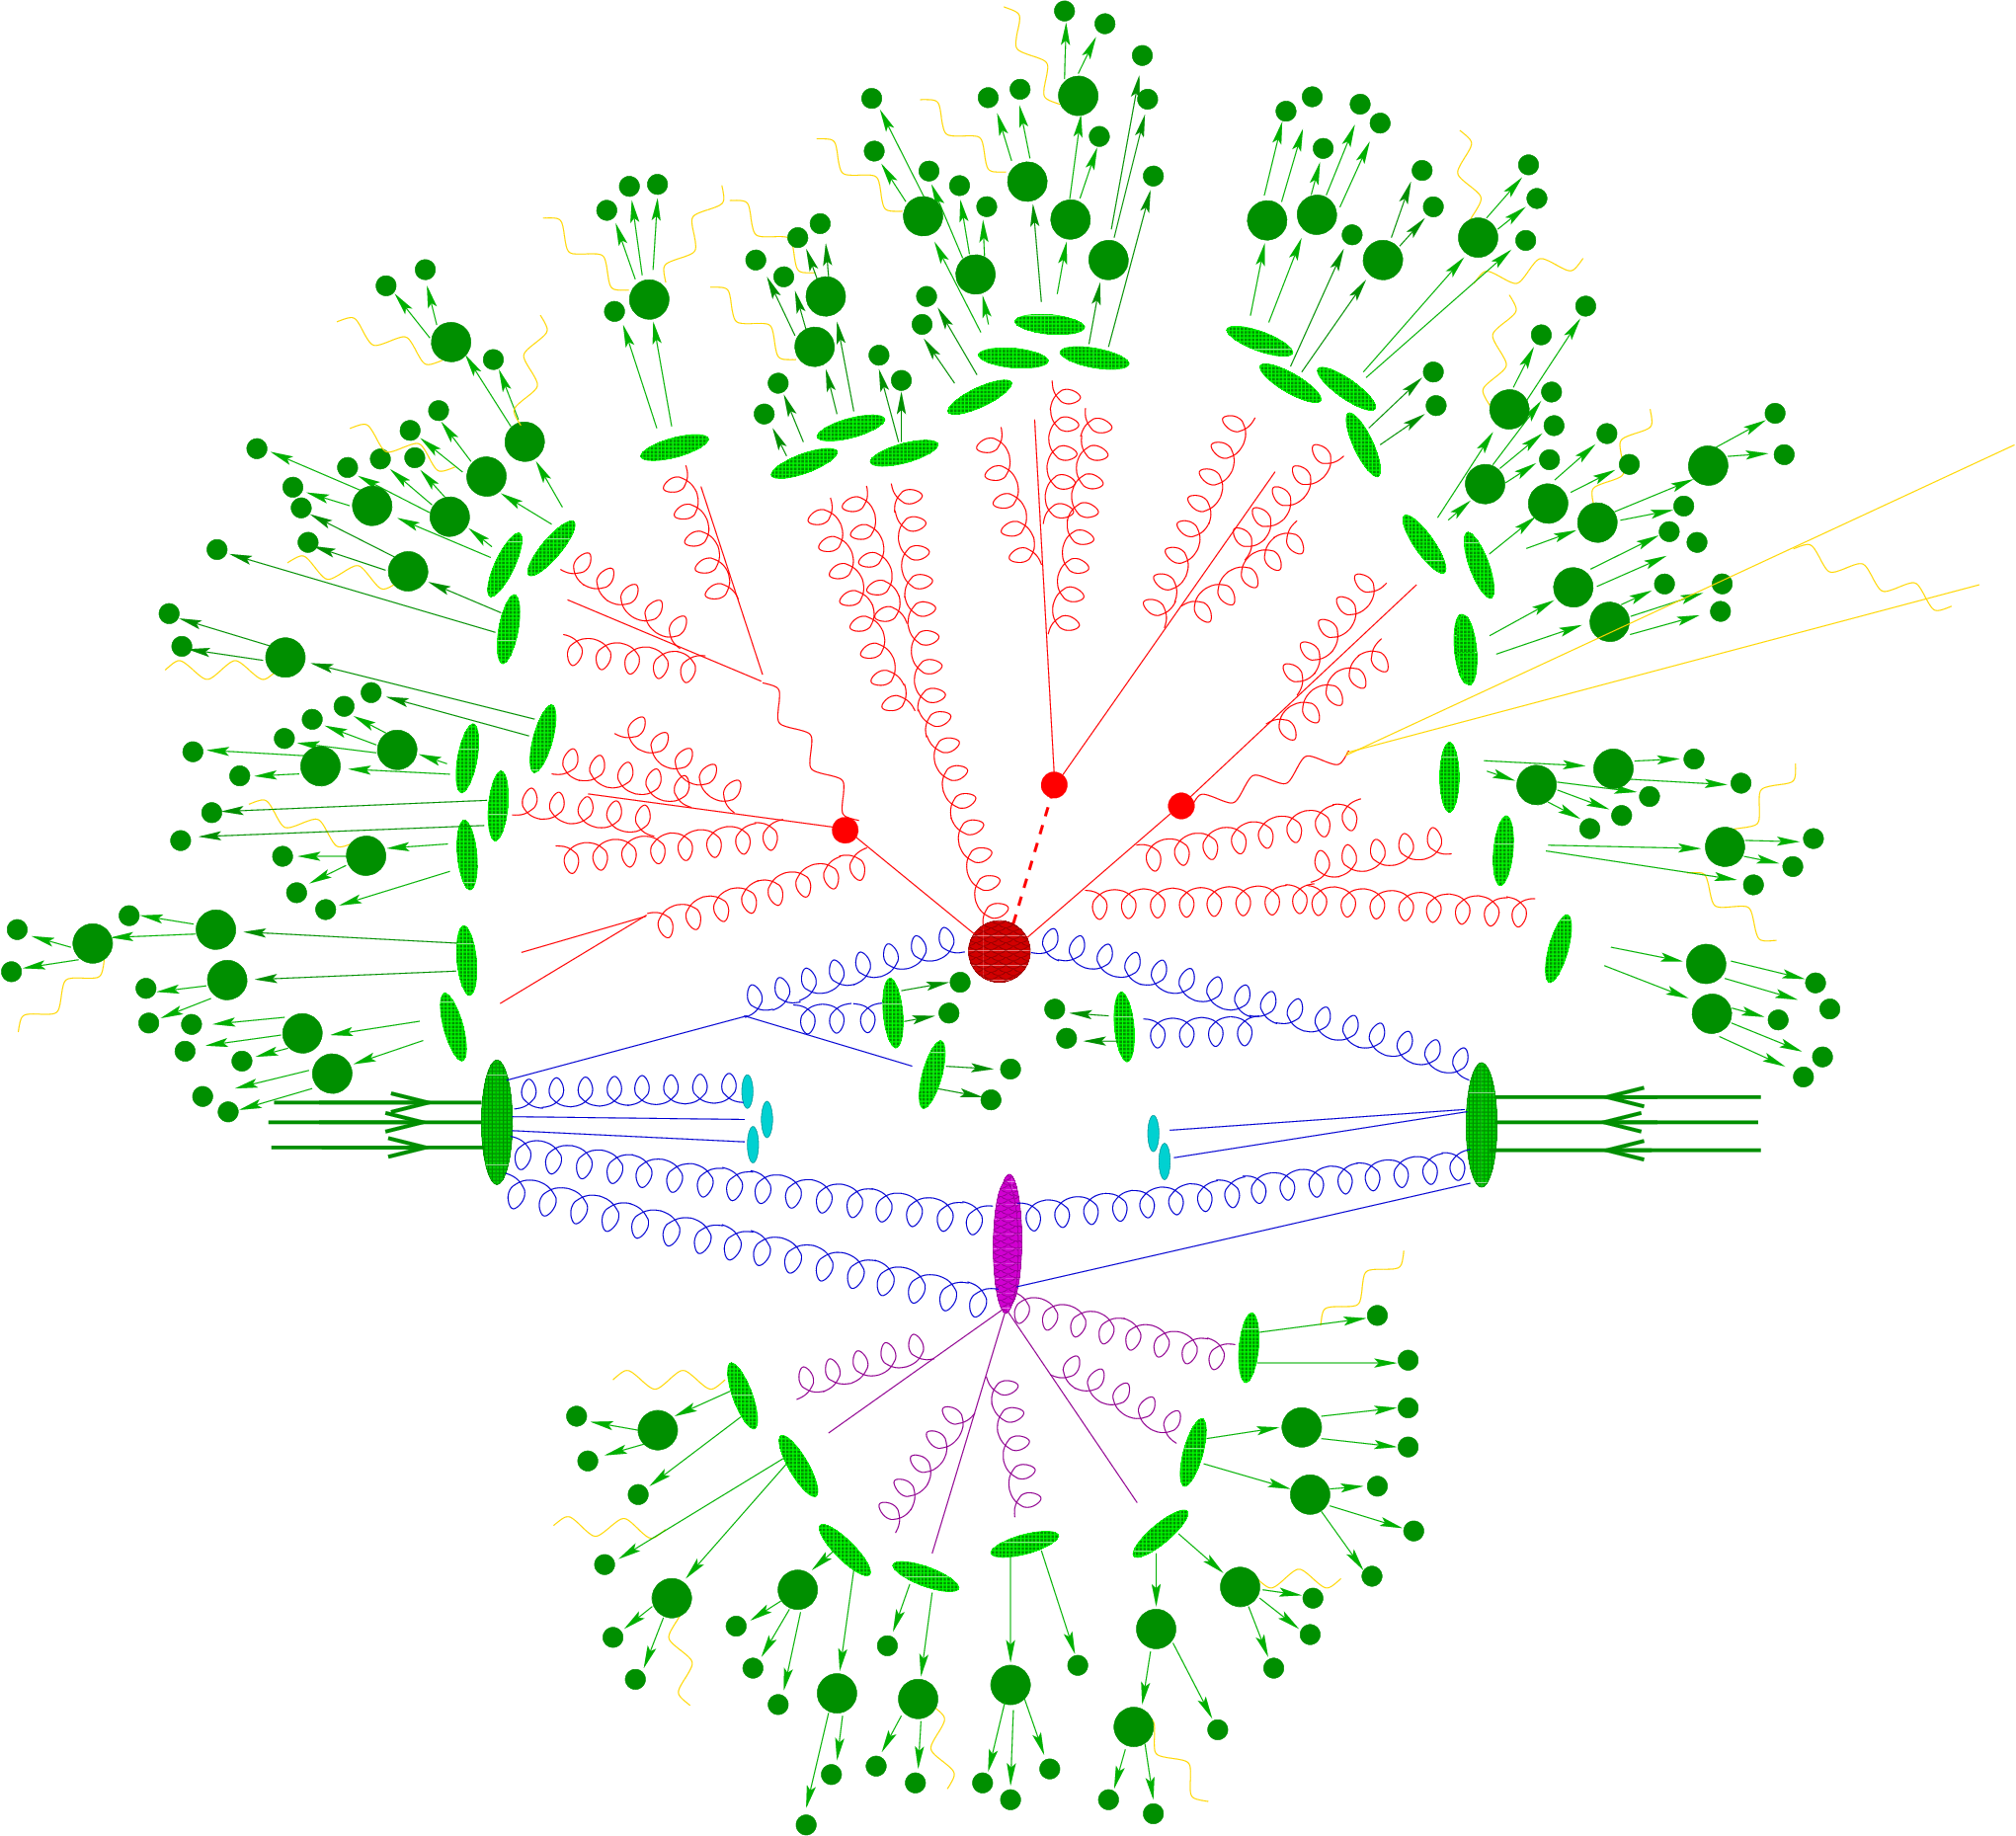
\includegraphics[width=.9\textwidth]{event.png} 
 \caption{Illustration of an event showing the hard scattering, parton shower, hadronisation, and underlying event. Figure taken from~\cite{Hoche:2014rga}.}
 \label{fig:event}
\end{figure}

\begin{itemize}
 \item[] \textbf{Hard scattering}\\
 In the hard interaction, two partons of the colliding protons, will interact with a certain probability at a given momentum transfer. This is parametrized by the \acp{PDF} $f(x, Q^2)$, were $x$ is the proton's momentum fraction and $Q^2$ is the momentum transfer scale. Experimentally determined \acp{PDF} are available from various groups, including e.g. CTEQ~\cite{Pumplin:2002vw}, MRST/MSTW~\cite{Martin:2009iq}, and NNPDF~\cite{Ball:2014uwa}. An example of such \acp{PDF} obtained by the NNPDF group is shown in Figure~\ref{fig:pdf}. This figure shows that the valence quarks in the proton, namely the up and down quarks it is made of, have a larger momentum fraction than the remaining sea quarks, which appear as virtual quark-antiquark pairs forming from from gluons and annihilate again, making them much less stable than the valence quarks. The \acp{PDF} are then convoluted with the matrix element of the hard scattering, which is the process of interest where the two colliding partons create high-energetic final state particles. This is done using an event generator, such as \textsc{MadGraph5\_}a\textsc{MC@NLO}~\cite{Alwall:2014hca} and \textsc{PowHeg}~\cite{Frixione:2007vw}. With \textsc{MadGraph5\_}a\textsc{MC@NLO} the matrix element can for many processes be calculated at tree-level or \ac{LO}, and since the addition of a\textsc{MC@NLO} at \ac{NLO} as well. This generator was used to produce most of the background processes for the Monojet analysis detailed in Chapter~\ref{ch:monojet} and for the \ac{SIMP} signal used in Chapter~\ref{ch:SIMPs}. \textsc{PowHeg} is able to generate events using \ac{NLO} computations, but only for a relatively limited number of physics processes. This generator was used to produce the monojet signal samples and the background processes from single-top production. Since \ac{NLO} calculations are more time-consuming, one can instead use the less precise method of scaling a \ac{LO} cross section to the \ac{NLO} level by using a so-called k-factor, defined as the ratio of the \ac{NLO} and \ac{LO} cross sections. However, these k-factors often need to be determined as a function of the relevant kinematic variables as they depend on the kinematic phase space and the probed energy scale.

\begin{figure}[ht]
  \centering
 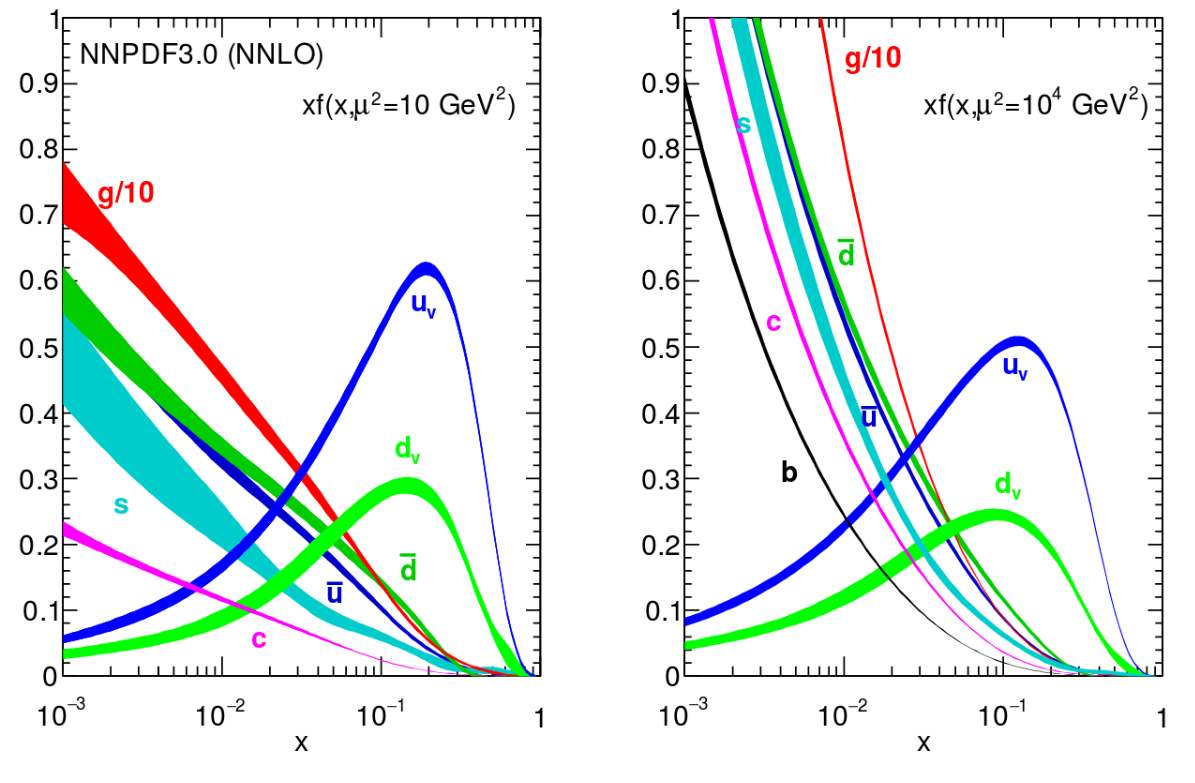
\includegraphics[width=.75\textwidth]{pdf.png} 
 \caption{The parton distribution functions multiplied by the momentum fraction $x$ at energy scales $Q^2 = \SI{10}{GeV^2}$ (left) and $Q^2 = \SI{10000}{GeV^2}$ (right), obtained in the NNLO NNPDF 3.0 global analysis. Figures taken from~\cite{Ball:2014uwa}.}
 \label{fig:pdf}
\end{figure}

 \item[] \textbf{Parton showering}\\
Since the colliding partons have a colour charge, the hard scattering will be accompanied by a cascade of radiation from \acs{QCD} processes. The partons will for example radiate soft gluons or split into two collinear partons. This radiation can originate from the incoming partons, which is referred to as \ac{ISR}, or the outgoing partons in the final state, the so-called \ac{FSR}. The perturbative evolution of the cascade can be modelled using the DGLAP (Dokshitzer-Gribov-Lipatov-Altarelli-Parisi) equations~\cite{Gribov:1972ri, Dokshitzer:1977sg, Altarelli:1977zs}. These equations describe the time evolution of the probability of a `mother' parton to split into `daughter' partons at an energy scale $Q^2$. The momentum of the mother is then divided among the daughter partons, which can in turn split into other partons at a lower $Q^2$ scale. The cascade continues down to an energy scale $\Lambda_{QCD}$ where the strong interaction becomes non-perturbative. The resulting number of jets can vary depending on the modelled process.
% , as shown in Figure~\ref{fig:njets}. {\color{red}Still need to describe figure, but it shows the opposite as expected for vector and scalar}
% 
% \begin{figure}[ht]
%   \centering
%  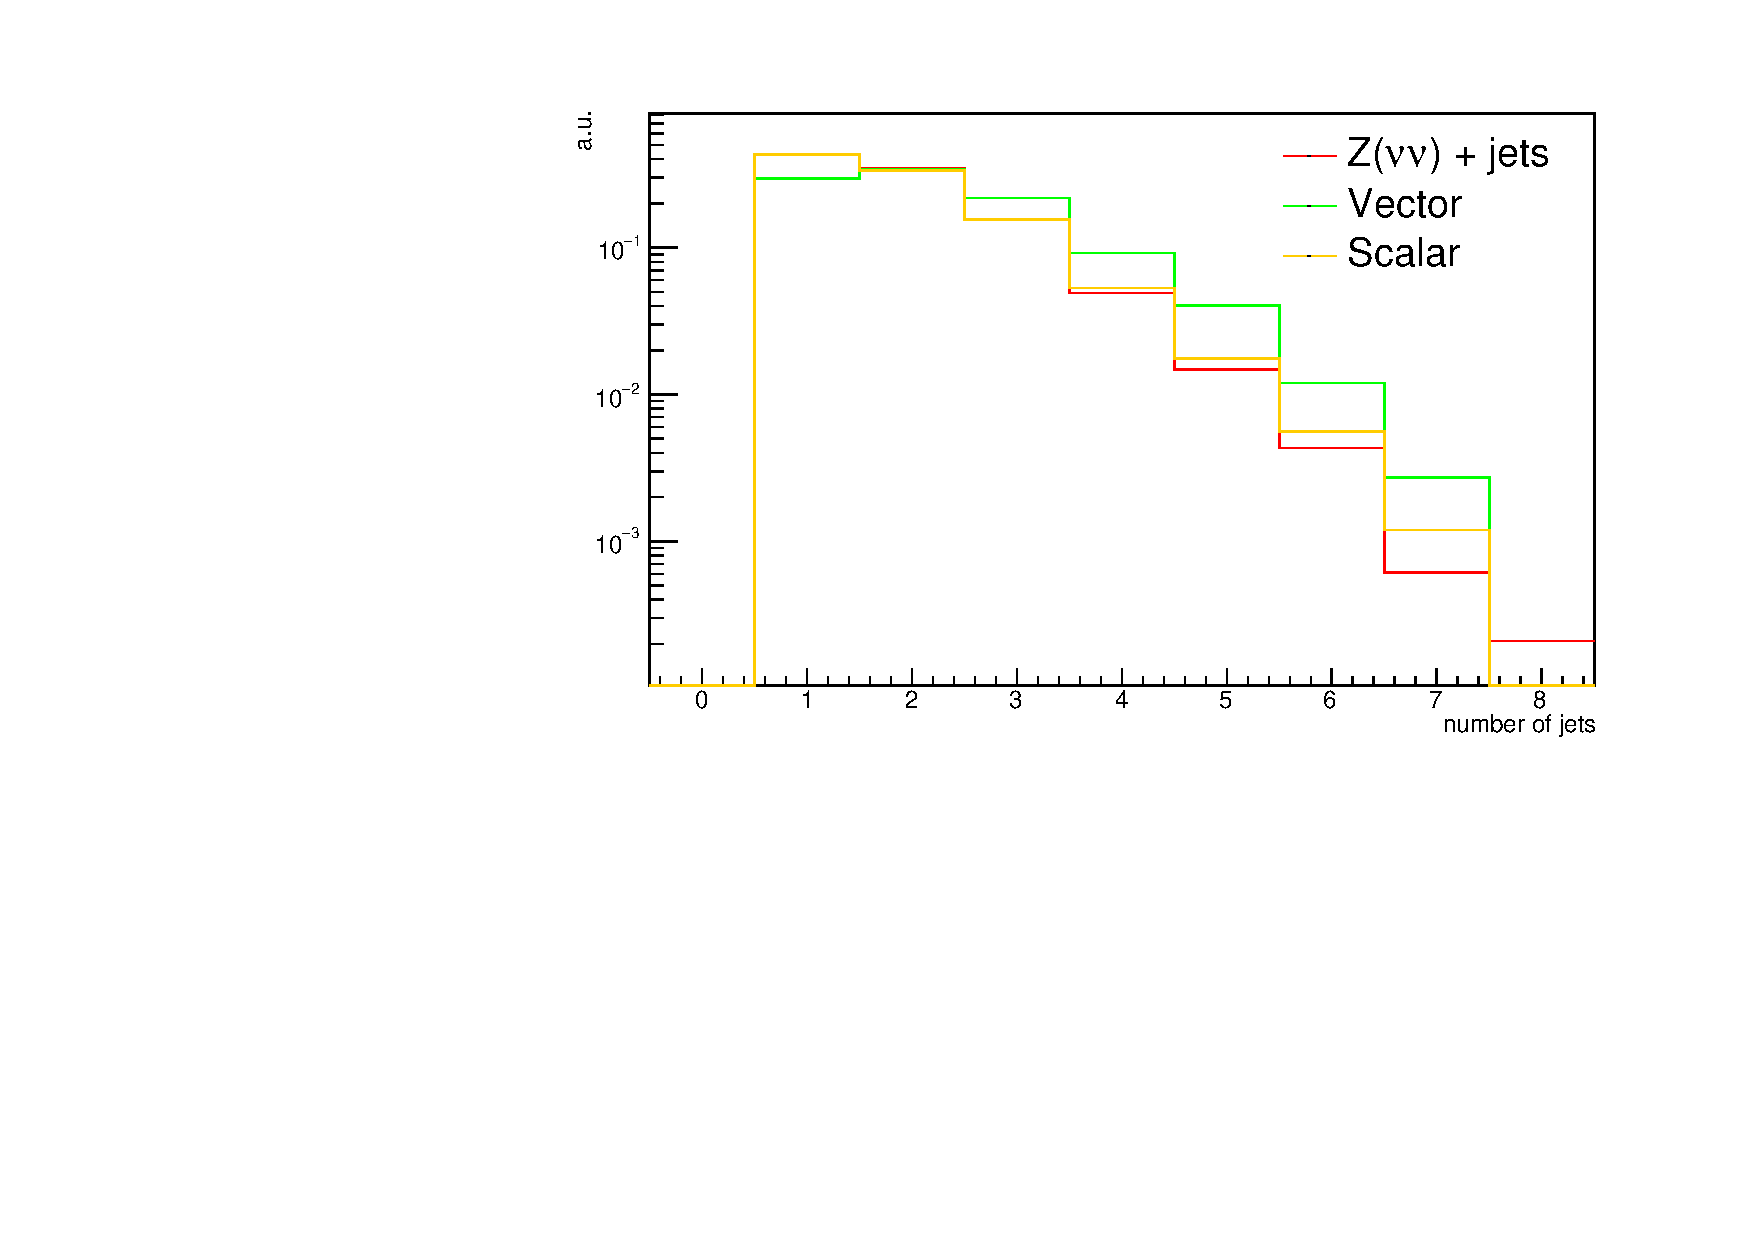
\includegraphics[width=.7\textwidth]{njets.pdf} 
%  \caption{.}
%  \label{fig:njets}
% \end{figure}

\item[] \textbf{Hadronisation}\\
The next step after the showering is the hadronisation of the coloured particles produced in the parton shower, transforming them into colour-neutral hadrons. Since this happens at low energy scales where the perturbative approach of \acs{QCD} is not valid, phenomenological models have to be used. For most of the processes considered in this thesis, the showering and hadronisation is done with \textsc{Pythia 8}~\cite{Sjostrand:2006za}, using a standard set of parameters which were tuned to reproduce the experimental data. In \textsc{Pythia}, the string Lund model~\cite{Andersson:1983ia} is used, based on string fragmentation. This model starts from the idea of a string connecting a quark $q$ and an antiquark $\bar{q}$, following the assumption of linear confinement. As the two quarks move away from each other, the string stretches and the potential energy stored in the string increases. The increase in potential energy is assumed to be proportional to the distance between the quarks. When the energy becomes sufficient to produce a new pair of quarks $q'\bar{q}'$ with mass $m$, the string breaks and the original quark pair is split into two new pairs, $q\bar{q}'$ and $q'\bar{q}$. If the invariant mass of the new strings is large enough, the same process is repeated, leading to a new break-up. This procedure continues until only colour-neutral hadrons with an on-shell mass remain.

\item[] \textbf{Additional activity in the event}\\
In addition to \ac{ISR} and \ac{FSR}, also beam remnants and multiple parton interactions give rise to additional activity in the event, referred to as the underlying event. After the partons participating in the hard scattering are extracted, the remainder of the protons have a non-zero colour charge. The creation of additional hadrons during the hadronisation is therefore possible. Multiple parton interactions represent additional interactions which can take place between other incoming partons. As the probability for an additional hard interaction to occur is rather small, the activity from multiple parton interaction is typically much less energetic than the hard interaction, producing mostly low energetic hadrons. Finally, additional collisions between other protons in the same bunch crossing, or from a previous or future bunch crossing, respectively referred to as in-time and out-of-time pileup, add extra activity in the event. The pileup distribution is for example shown in Figure~\ref{fig:pileup} for QCD dijet events recorded in 2016, and is compared to simulated QCD events. This shows that there were about $20$ collisions per bunch crossing on average. Typically, the simulation does not completely agree with the data and needs to be reweighted in order to match the data.

\begin{figure}[ht]
  \centering
 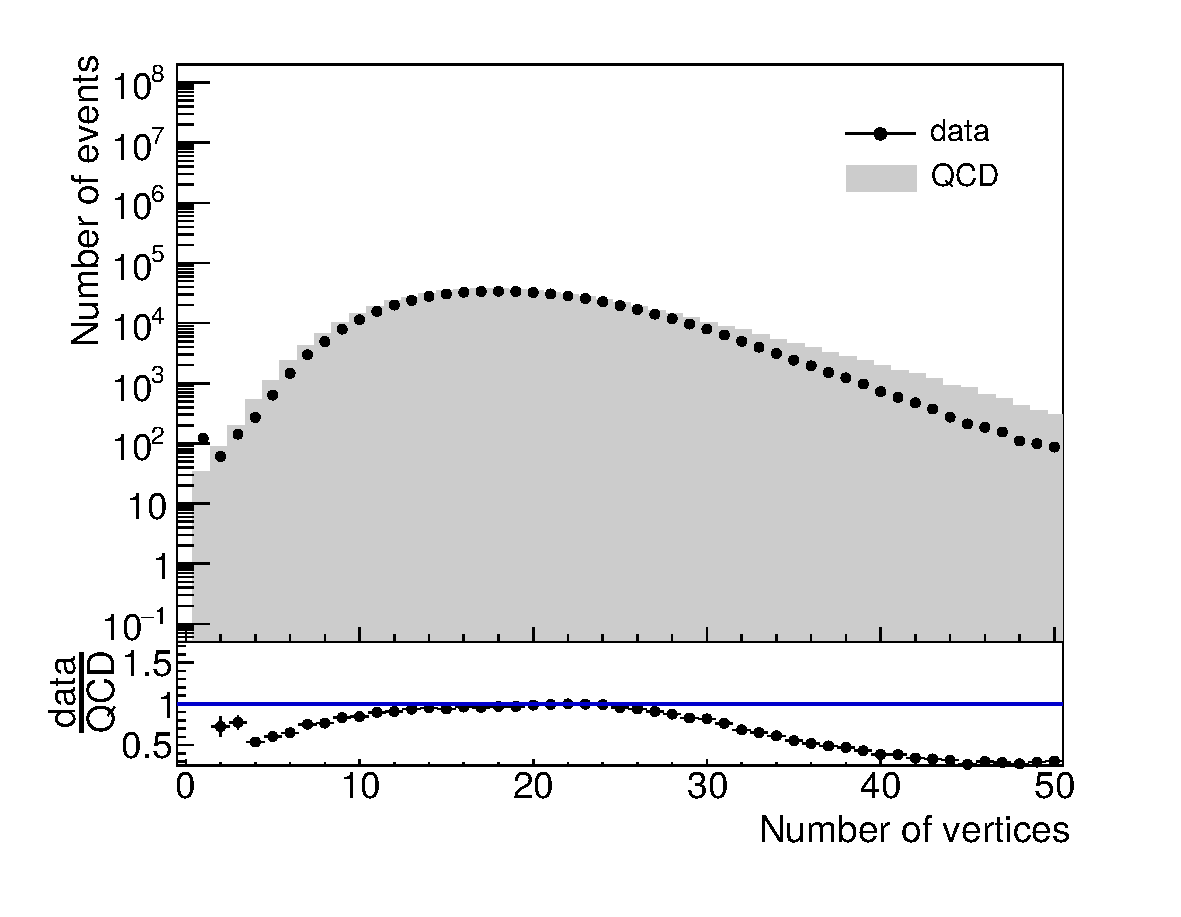
\includegraphics[width=.75\textwidth]{pileup.pdf} 
 \caption{The distribution of the number of vertices for \ac{QCD} dijet events recorded in 2016 compared to simulated \ac{QCD} events.}
 \label{fig:pileup}
\end{figure}
 \end{itemize}

\subsection{Generation of the monojet signals}
\label{sec:monojet_sim}

In the monojet analysis, the simplified models described in Section~\ref{sec:monojet_models} are considered. The used signal samples were generated with \textsc{PowHeg}, which can generate \ac{NLO} vector and axial-vector mediator production and \ac{LO} scalar and pseudoscalar production. The samples were also produced at \ac{LO} with MCFM~\cite{Campbell:2010ff} as a cross check. The scanned mediator masses are $m_{\phi} = 10, 20, 50, 100, 200, 300, 500,$ $ 1000, 2000,$ \SI{10000}{GeV}, for dark matter masses of $m_{\chi} = 1, 10, 50, 100, 150, 500, \SI{1000}{GeV}$, with $m_{\chi} \leq m_{\phi}$.

\subsection{Generation of the SIMP signal}
\label{sec:simp_sim}

For the generation of the \ac{SIMP} signal, the model Lagrangian given in equation~\ref{eq:SIMP_lagrangian} is implemented in \textsc{FeynRules 2.0}~\cite{Alloul:2013bka}. The matrix element is then calculated at \ac{LO} and events are generated using \textsc{Madgraph 5}. The subsequent parton shower and hadronisation is done with \textsc{Pythia 8}, using tune CUEP8M1. Several samples were produced, with \ac{SIMP} masses $m_{\chi} = 1, 10, 100, 200, 400, 700,$ \SI{1000}{GeV}. The corresponding productions cross sections are given in Table~\ref{tab:signal_samples}. 

\begin{table}[ht]
  \centering
\caption{Production cross section for each \ac{SIMP} mass, after $|\eta_{\chi}| < 2.5$ and $p_{\rm T}^{\chi} > 200$ GeV generator level cuts.}
\begin{tabular}{| c | l |}
\hline
$m_\chi$ [GeV] & $\sigma_{\bar{\chi}\chi}$ [pb] \\
\hline
    1 &  4.46 \\
  10 &   4.40  \\
  100 &  2.55  \\
  200 &   0.790  \\
  400 &   0.0743   \\
  700 &   0.00485  \\
1000 &   0.000571  \\
\hline
\end{tabular}
\label{tab:signal_samples}
\end{table}

\section{Detector simulation}
\label{sec:sim}

After being generated, the collision events are passed on to the \ac{CMS} detector simulation, which is based on the \textsc{Geant 4}~\cite{Allison:2006ve} simulation toolkit. This toolkit provides a description of the interaction between particles and the detector material, including effects such as bremsstrahlung of charged particles, photon conversions, energy loss of charged particles by ionization, and the showering of electrons, photons and hadrons in the calorimeters due to interaction with the material. The \ac{CMS} simulation package contains the geometry of the detector with all the sensitive layers designed to detect the traversing particles, as well as the dead material regions consisting of e.g. support structures, cables and cooling pipes. A precise map of the magnetic field is also included in order to simulate the curvature of the charged particles correctly.

Next, the impact of the detector, coming from the electronic response produced by the hits in the active detector material, the digitization, the data transmission, and any reconstruction performed in the electronics such as zero-suppression or cluster reconstruction, is simulated. In this way, an event content similar to the output of the real detector is obtained. At this point the effect of pileup is also included by adding detector hits of generated proton-proton interactions on top of the hits resulting from the main interaction. Most of the simulated event samples used in this thesis are processed using this detector simulation. However, the interaction of new particles that can arise from specific theory models is not always readily described in \textsc{Geant}. This is the case for the signal samples used in the analysis described in Chapter~\ref{ch:SIMPs}, so an additional step was needed in order to simulate \acfp{SIMP} in the \ac{CMS} detector, described in Section~\ref{sec:SIMPs}. 

\section{Event reconstruction}
\label{sec:reconstruction}

Once the detector response has been simulated, the obtained events can be reconstructed. The same method is applied for these simulated events and for data coming from the detector. First, the reconstruction of tracks is performed, with a specific track reconstruction for electrons and muons. Furthermore, the calorimeter deposits, generated by electrons, photons, and hadrons, are grouped into clusters. Additionally, the reconstruction is further improved by using the so-called \acf{PF} algorithm described in Section~\ref{sec:PF}. This algorithm greatly improves the performance for jet and hadronic $\tau$ decay reconstruction, missing transverse momentum determination, as well as electron and muon identification. Finally, the obtained \ac{PF} candidates are clustered into jets, and the missing transverse energy can be derived.

\subsection{Track and vertex reconstruction}
\label{sec:tracking}

The tracks of charged particles going through the \ac{CMS} tracker are reconstructed with an iterative tracking approach. This is used to cope with the high occupancy of hits and consequently high combinatorics. Additionally, the first iterations search for tracks with less possible combinations, such as tracks with many pixel hits or a high momentum. After every iteration, the hits associated with the found track are removed to reduce the combinatorics. Each iteration consists of four steps:
\begin{enumerate}
 \item \textbf{Seed generation.} In this first step hits are combined into seeds for the subsequent track finding. In the initial iterations pixel triplets are used, then pixel pairs together with a constraint on the origin of the trajectory based on the assumption that it originated near the beam spot, in order to take gaps or non-working modules into account. Next, mixed pixel/strip triplets are taken, and finally strip-only seeds are used. These additional iterations improve the acceptance in $p_T$ and in displacement with respect to the primary vertex.
 \item \textbf{Track finding}. The seeds are used as starting point for a Kalman filter algorithm. This method extrapolates the seed trajectory outward to the next layer, taking into account the presence of the magnetic field, potential energy loss and multiple scattering. If compatible hits are found in the next layer, the parameters of the trajectory are updated. This process continues until the outermost layer of the tracking system. Using this method, a given seed can generate multiple tracks, or different tracks can share hits. A trajectory cleaner therefore determines the fraction of hits the tracks have in common and discards the track with the lowest number of hits when there are too many shared hits. If both tracks have the same number of hits, the track with the largest $\chi^2$ value is removed.
 \item \textbf{Track fitting.} The track parameters are then refitted using a Kalman filter and smoother, taking all hits determined in the track finding step into account. This is done in order to find the optimal track parameters.
 \item \textbf{Track selection.} Finally, the tracks are selected based on quality requirements, such as the number of layers that have hits, the $\chi^2/$dof, and the distance to a primary vertex. This greatly reduces the fraction of reconstructed tracks that are fake.
\end{enumerate}

The performance of the track reconstruction is excellent, and a high track-finding efficiency is obtained~\cite{Chatrchyan:2014fea} while keeping the rate of fake tracks negligible. The highest tracking efficiency is obtained for muons, which traverse the full detector volume and have an improved momentum resolution at high $p_T$ due to tracking information from the muon detectors giving a long lever arm. For isolated muons with $p_T$ between 1 and \SI{100}{GeV} the tracking efficiency is higher than 99\% for the entire $\eta$ coverage of the tracker, as can be seen from the left plot in Figure~\ref{fig:eff_eta}. The $p_T$ resolution is about 2-3\% for a muon with $p_T = $ \SI{100}{GeV} up to $|\eta| < 1.6$, but worsens for higher pseudorapidities. Different types of particles interact differently with the detector material. Charged hadrons, for example, are also subject to elastic and inelastic nuclear interactions and have a tracking efficiency of 80-95\% depending on pseudorapidity and transverse momentum, as shown in the right plot of Figure~\ref{fig:eff_eta}.

\begin{figure}[ht]
  \centering
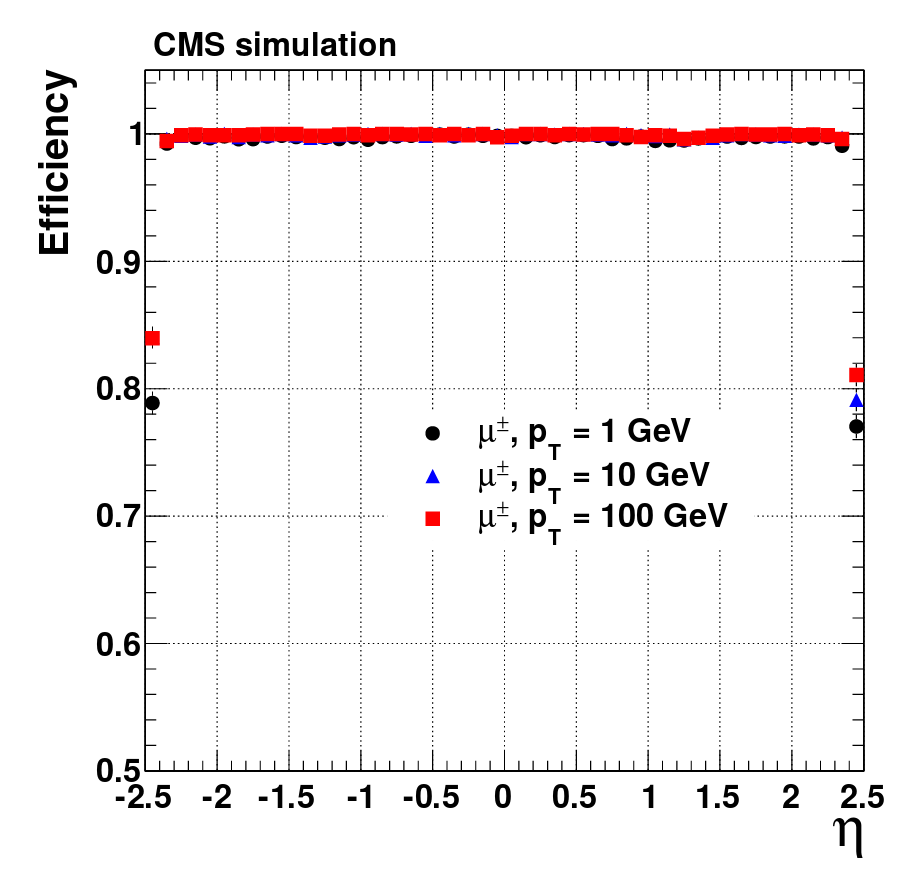
\includegraphics[width=.4\textwidth]{muon_eff_eta}\hspace{1cm}
 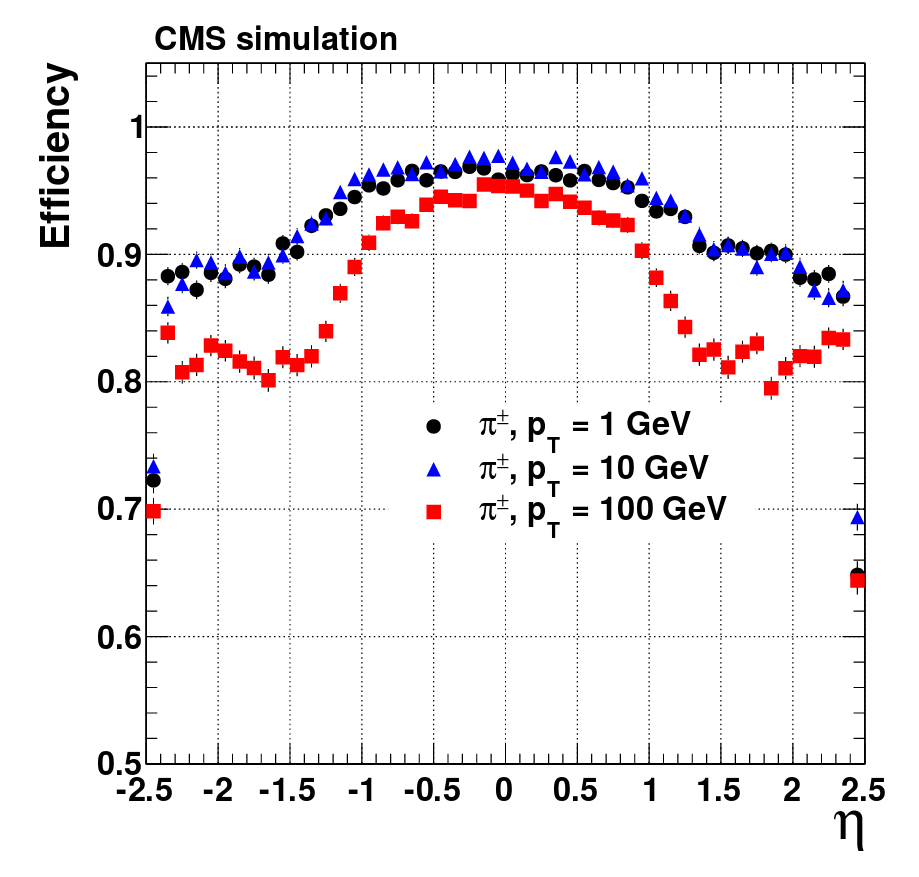
\includegraphics[width=.4\textwidth]{pion_eff_eta} 
 \caption{The muon efficiency (left) and pion efficiency (right) as a function of pseudorapidity, for multiple transverse momenta. Figures taken from~\cite{Chatrchyan:2014fea}}
 \label{fig:eff_eta}
\end{figure}

Finally, the primary vertices are reconstructed from the tracks. Since the collisions happen between bunches of protons, at the luminosities reached at the \ac{LHC} multiple protons will be colliding at the same time. The particles generated in these pileup interactions are all detected simultaneously and form a challenge to disentangle them from the particles coming from the to be studied interaction.

% The reconstruction is done in 2 steps: first the tracks that appear to originate from the same interaction vertex are clustered, then a fitting procedure computes the vertex parameters and assigns a weight to each associated track, reflecting the probability that it corresponds to the considered vertex. Figure~\ref{fig:PV} shows the reconstruction efficiency and the resolution of the primary vertex. The more tracks, the better the vertex is constrained and thus the better the resolution.

The reconstruction is performed as detailed in Section~9.4.1 of~\cite{CMSCollaboration:2015zni}, by first clustering the tracks based on their $z$ coordinate at the point of closest approach to the beam line. The vertex position is then estimated using an adaptive vertex fit~\cite{Fruhwirth:2007hz} with as input the collection of tracks that is expected to come from the same interaction. Next, the tracks originating from the same vertex are clustered into jets with the anti-$k_T$ algorithm described in Section~\ref{sec:jet_reconstruction} using a distance parameter of 0.4.

% \begin{figure}[ht]
%   \centering
% 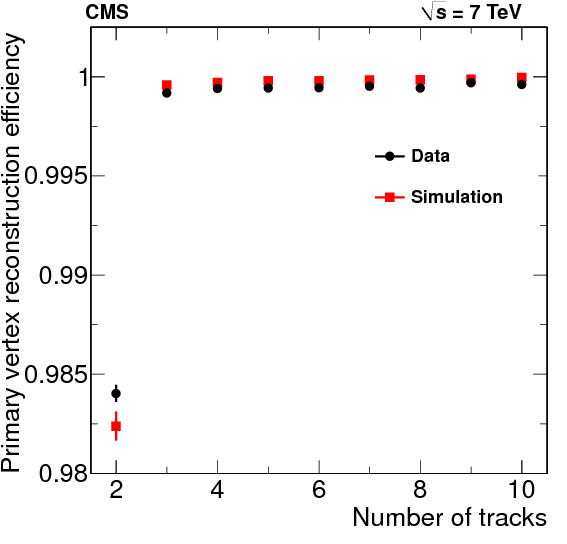
\includegraphics[width=.4\textwidth]{PV_eff}\hspace{1cm}
%  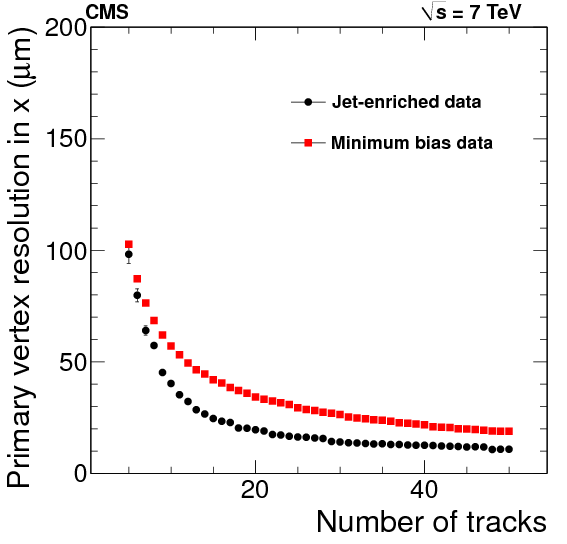
\includegraphics[width=.4\textwidth]{PV_res} 
%  \caption{The primary vertex reconstruction efficiency (left) and resolution (right) as a function of the number of tracks associated to it. Figures taken from~\cite{Chatrchyan:2014fea}}
%  \label{fig:PV}
% \end{figure}

The vertex with the highest $\sum p_T^2$ is chosen as primary vertex, where the sum runs over these reconstructed jets, as well as the remaining tracks associated to the vertex and the missing transverse momentum at this vertex, in order to take into account neutral particles.
%tracks associated to the vertex following the application of a deterministic annealing filter which assigns weights to sufficiently high-quality tracks that enter the vertex fit~\cite{Chatrchyan:2014fea}. 
While in events with jets many tens of high-momentum tracks can usually be associated to a primary vertex, thus making primary vertex finding almost fully efficient and pure, in the case of a pair of neutral jets, produced for example by \acp{SIMP}, this is not the case any more. The underlying event and potentially initial state \acs{QCD} radiation can still provide some tracks, but in extreme cases a wrong vertex is chosen, arising from a hard pileup collision.

\subsection{Electron and isolated photon reconstruction}
\label{sec:electron_reconstruction}

Electrons are reconstructed using information from both the tracker and the calorimeters. Due to the large amount of material present in the tracker, electrons will emit bremsstrahlung photons, and photons will often convert into $e^+e^-$ pairs, which can again radiate bremsstrahlung photons.

For electrons, a \ac{GSF}~\cite{Strandlie:2006gi} candidate is taken as starting point. This \ac{GSF} candidate is obtained using 2 different methods to reconstruct the electron track from the hits in the tracker, which should gather all radiated energy from the electron. First, the ECAL-based approach is used, grouping \ac{ECAL} clusters into superclusters. These superclusters collect the energy of the electron and the bremsstrahlung photons in a small $\eta$ window and a large $\phi$ window, taking the bending of the electron track in the magnetic field into account. The supercluster energy and position is then used to estimate the position of the corresponding hits in the tracker layers. Subsequently, the tracker-based approach is used to find electrons missed by the ECAL-based method. In this case, the tracks from the iterative tracking with transverse momentum larger than \SI{2}{GeV} are used. Additional requirements are placed on the number of hits and the $\chi^2$ of the fit, and the specific electron tracking is performed, using a \ac{GSF} fit, which is more adapted to electrons than the Kalman filter used in the iterative tracking, as it describes the energy loss in each tracker layer. The electron seeds obtained with both methods are merged and used as input for the full electron tracking. The obtained electron tracks are then linked to \ac{ECAL} clusters by the \ac{PF} algorithm, as described in Section~\ref{sec:PF}. In the case of isolated photons, a candidate is seeded from an \ac{ECAL} supercluster with transverse energy larger than \SI{10}{GeV} which is not linked to a \ac{GSF} track.

The total energy of the accumulated \ac{ECAL} clusters is corrected for the energy that was lost in the process of reconstruction, using analytical functions of the energy and pseudorapidity. The applied corrections can be as large as 25\%, at low transverse momentum and at $|\eta| = 1.5$, where the material density in the tracker is largest. The energy of the electron is then obtained from a combination of the corrected energy and the momentum of the \ac{GSF} track, while the direction of the electron is taken from the \ac{GSF} track. For photons, the corrected energy and the direction of the supercluster are used.
% 
%  while for photons the candidates must be isolated from other tracks and calorimeter clusters, and the energy distribution in the \ac{ECAL} and the ratio between the \ac{HCAL} and \ac{ECAL} energies must be compatible with the expectation from a photon shower.

\subsection{Electron and photon identification}
\label{sec:electron_ID}

In general, the electron and photon candidates must satisfy identification criteria to be retained. In the case of electrons two methods for identification are available: a cut-based identification or a multivariate boosted decision tree (BDT) combining fourteen variables including the amount of energy radiated and the ratio between the energies gathered in HCAL and ECAL. In the monojet analysis described in Chapter~\ref{ch:monojet}, the former is used. In this method, four different working points are defined, denoted as ``tight'', ``medium'', ``loose'', and ``veto'', with varying signal efficiency and background rejection. For the electron veto the loose selection is used, while a tight identification is required on one electron to select the events in the dielectron and single electron control regions.

\renewcommand{\arraystretch}{1.1}
\begin{table}[ht!]
\centering
\small
\caption{Loose and tight electron identification criteria. The isolation is computed in a cone of $\Delta R < 0.3$ around the electron.}
\begin{tabular}{|l|l|l||l|l|c|}
\hline
\multirow{2}{*}{variable}                             &  \multicolumn{2}{c||}{loose} &  \multicolumn{2}{c|}{tight} \\
\cline{2-5}
                                                            &  barrel        & endcaps  &  barrel  & endcaps\\
\hline
full 5x5 $\sigma_{i\eta i\eta}$                             & $< 0.0114  $     & $< 0.0352  $ & $< 0.0101  $     & $< 0.0279  $ \\
$|\Delta \eta_{in}|$                                        & $< 0.0152  $     & $< 0.0113  $ & $< 0.00926 $     & $< 0.00724 $ \\
$|\Delta \phi_{in}|$                                        & $< 0.216   $     & $< 0.237   $ & $< 0.0336  $     & $< 0.0918  $ \\
H/E                                                         & $< 0.181   $     & $< 0.116   $ & $< 0.0597  $     & $< 0.0615  $ \\
relative isolation			                    & $< 0.126   $     & $< 0.144   $ & $< 0.0354  $     & $< 0.0646  $ \\
$|1/E - 1/p|\ [\mathrm{GeV}^{-1}]$                          & $< 0.207   $     & $< 0.174   $ & $< 0.012   $     & $< 0.00999 $ \\
$|\mathrm{d_{xy}(vtx)}|$ [cm]                               & $< 0.0564  $     & $< 0.222   $ & $< 0.0111  $     & $< 0.0351  $ \\
$|\mathrm{d_{z}(vtx)}|$ [cm]                                & $< 0.472   $     & $< 0.921   $ & $< 0.0466  $     & $< 0.417   $ \\
expected inner missing hits                                 & $\leq 2$         & $\leq 3$     & $\leq 2$           & $\leq 1$   \\
pass conversion veto                                        & yes              & yes          & yes              & yes        \\
\hline
\end{tabular}
\label{tab:ElectronID}
\end{table}

Similarly, for the photons, both a cut-based identification and a multivariate analysis can be used. Both for the monojet and the \ac{SIMP} analysis, described in Chapters~\ref{ch:monojet} and \ref{ch:SIMPs}, the cut-based identification is used. Three standard working points are provided, denoted as ``loose'', ``medium'', and ``tight'', with an average efficiency of 70\%, 80\%, and 90\%, respectively. In both analyses, the loose identification is used for the photon veto. In the \ac{SIMP} analysis, the event is only rejected when the identified photon is within a cone of $\Delta R < 0.1$ of one of the two leading jets. Additionally, the photon veto is extended to reject events containing jets with a large photon energy fraction and unidentified photons. This happens for instance when there is a photon conversion in the tracker. The event is therefore rejected when the jet photon energy fraction is larger than 0.8, the photon is not identified by the loose criteria, and a conversion is matched to the photon within $\Delta R < 0.2$ and has $p_{T,conv} / p_{T,\gamma} > 0.3$. Lastly, the two jets are also required to have a neutral electromagnetic energy fraction lower than 0.9, corresponding to one of the standard tight jet identification requirements mentioned in Section~\ref{sec:jet_reconstruction}. Finally, the monojet analysis uses a photon + jets control region as well. These events are selected by applying the tight photon identification.


\renewcommand{\arraystretch}{1.1}
\begin{table}[ht!]
\centering
\footnotesize
\caption{Loose and tight photon identification criteria. The isolation is computed in a cone of $\Delta R < 0.3$ around the photon.}
\begin{tabular}{|l|l|l||l|c|}
\hline
\multirow{2}{*}{variable}                             &  \multicolumn{2}{c||}{loose} & tight \\
\cline{2-4}
                                                            &  barrel        & endcaps  &  barrel  \\
\hline
full 5x5 $\sigma_{i\eta i\eta}$            & $< 0.0102$                                                  & $< 0.0274$    & $< 0.0102$     \\
H/E                                        & $< 0.05$                                                    & $< 0.05$     & $< 0.05$      \\
charged hadron                   & \multirow{2}{*}{$< 3.32$}  & \multirow{2}{*}{$< 1.97$}    & \multirow{2}{*}{$< 1.37$}    \\
 isolation        &     &      &   \\
neutral hadron  & $< 1.92 + 0.014\times p_T$ & $< 11.86 + 0.0139\times p_T$ & $< 1.06 + 0.014\times p_T$  \\
isolation          & $\quad +1.9\times 10^{-5} \times {p_T}^2$  & $\quad +2.5\times 10^{-5} \times {p_T}^2$ & $\quad +1.9\times 10^{-5} \times {p_T}^2$ \\
photon isolation                           & $< 0.81 + 0.0053\times p_T$                                 & $< 0.83 + 0.0034\times p_T$ & $< 0.28 + 0.0053\times p_T$   \\
conversion safe             & \multirow{2}{*}{yes}                                                         & \multirow{2}{*}{yes}        & \multirow{2}{*}{yes}       \\
electron veto              &      &   &  \\
\hline
\end{tabular}
\label{tab:PhotonID}
\end{table}

\subsection{Muon reconstruction}
\label{sec:muon_reconstruction}

Muon tracking is performed using 2 complementary approaches. The first method starts from standalone muons, which are reconstructed from hits in the muon detectors only using pattern recognition. The standalone muons are then matched to tracks in the tracker, and the hits are combined to form a global muon track. This global muon fit improves the momentum resolution compared to the tracker-only fit at muon momenta larger than \SI{200}{GeV}.

For momenta below \SI{10}{GeV}, muons often fail the global muon conditions which require the muon to penetrate through more than one muon detector plane, due to the large multiple scattering in the return yoke. In this case, tracker-only muon reconstruction is more efficient since it only requires one muon segment. Each track in the tracker with a transverse momentum larger than \SI{0.5}{GeV} and a total momentum larger than \SI{2.5}{GeV} is therefore extrapolated to the muon system and if at least one matching track segment is found, it is retained as muon candidate.

Within the geometrical acceptance of the muon system about 99\% of the muons are reconstructed, either as global muon or as tracker muon and frequently as both. Global and tracker muons that share the same track inside the tracker are merged into a single candidate. Muons that are only reconstructed as standalone muons have a worse momentum resolution compared to the global and tracker muons. These standalone muons are however only considered in the further reconstruction when the fit is of high quality and is associated with a large number of hits in the muon system.

Charged hadrons can be misreconstructed as muons if e.g. a part of the hadron shower reaches the muon system. In order to improve the muon identification, the \ac{PF} muon identification algorithm described in Section~\ref{sec:PF} also matches energy deposits in the \ac{ECAL} and \ac{HCAL} with the muon track.

\subsection{Muon identification}
\label{sec:muonID}

When using muons for physics analysis, some identification criteria are generally applied in order to ensure the quality of the muons. There are several standard levels of identification, denoted as ``tight'', ``medium'', and ``loose'', which provide a trade-off between muon identification efficiency and misidentification. In general, the tight and loose identification are the most widely used identification criteria.

The loose identification only requires the muons to be either global or tracker-only muons, and to be identified by the \ac{PF} algorithm as a muon. As a result, it is highly efficient for both prompt muons and muons from quark decays. In analyses with prompt muons, this identification is therefore often complemented by an impact parameter cut, associating the muon to the primary vertex.

For the tight identification, the muon is required to be a global muon and to be identified by the \ac{PF} algorithm as a muon. The normalized $\chi^2$ of the global muon track fit should be smaller than 10 to suppress hadronic punch through and muons from hadron decays in flight. To further suppress these contributions at least one muon chamber hit should be included in the global muon track fit and muon segments should be found in at least two muon stations. Cosmic muons and tracks from pileup are suppressed by requiring the tracker track to have $|d_{xy}| < \SI{2}{mm}$ and $|d_z| < \SI{5}{mm}$, with $d_{xy}$ the traverse impact parameter and $d_z$ the longitudinal distance with respect to the primary vertex. Finally, at least one pixel hit is required, as well as hits in at least 5 tracker layers, in order to ensure a good $p_T$ measurement.

In the case of the monojet analysis described in Chapter~\ref{ch:monojet}, the loose muon identification is used to select muons for the muon veto. An additional isolation cut of 0.2 is applied in order to reject muons inside jets. The isolation value is computed as the sum of the transverse momenta of all charged hadrons associated to the primary vertex, neutral hadrons, and photons in a cone of $\Delta R < 0.4$ around the muon, relative to the $p_T$ of the muon. The tight muon identification is used as well, to select events in the dimuon and single muon control regions. 

\subsection{Particle flow}
\label{sec:PF}

The \acf{PF} algorithm~\cite{CMS-PRF-14-001} reconstructs so-called particle flow candidates by combining information from all different \ac{CMS} subdetectors, linking different elements, such as tracks in the tracker, calorimeter clusters, and muon tracks. A global picture of the event is thus formed, where each particle is uniquely identified. The obtained collection of particle candidates is subsequently used to reconstruct jets and tau leptons, and to determine the missing transverse momentum.

In a first step, the \ac{PF} algorithm identifies charged particle tracks, as defined in Section~\ref{sec:tracking} for all tracks, and in Sections~\ref{sec:electron_reconstruction} and \ref{sec:muon_reconstruction} for electron and muon tracks in particular. At the same time, the calorimeter clusters are reconstructed with a clustering algorithm designed specifically for the \ac{PF} event reconstruction. In this algorithm, cluster seeds are first identified as local energy maxima with respect to the four or eight closest cells, if the energy deposited in the cell is above a given seed threshold. The clusters are then formed by accumulating neighbouring cells with an energy above a given cell threshold, suppressing noise.

The \ac{PF} elements in the different subdetectors are then connected by a link algorithm which avoids any double counting. The link algorithm produces blocks of associated elements, quantifying the quality of the link by defining a geometrical distance between the elements. When an element is linked to multiple other elements, only the link with the shortest distance is kept. More precisely, a link between a track in the tracker and a calorimeter cluster is made by extrapolating it from the last hit in the tracker to the calorimeters. The distance between the position of the extrapolated track and the cluster in the ($\eta$, $\phi$) plane is then used to define the link distance. At the interaction points between the track and the tracker layers, tangents to the \ac{GSF} tracks are extrapolated to the \ac{ECAL} in order to collect the energy of photons radiated by electron bremsstrahlung. A dedicated conversion finder was also developed to identify bremsstrahlung and prompt photon conversions into $e^+e^-$ pairs. Links between calorimeter clusters are established outside of the tracker acceptance, or between the preshower and \ac{ECAL} clusters in the preshower acceptance. In this case the link distance is also defined as the distance between the position of the clusters. Charged particle tracks can also be linked by a common secondary vertex. Finally, the \ac{PF} muon identification algorithm associates the muon tracks to the muon energy deposits in the \ac{ECAL} and \ac{HCAL}, to improve the muon identification performance.

In a next step, the \ac{PF} blocks obtained by linking the multiple \ac{PF} elements, are classified as muons, electrons, or isolated photons. The corresponding elements are then excluded from further consideration. Once electrons, muons, and isolated photons have been identified, the remaining elements are identified as charged hadrons, neutral hadrons, or photons produced in jets. Within the tracker acceptance, the \ac{ECAL} clusters not linked to any track are classified as photons, while the clusters in the \ac{HCAL} without a matched track are labelled as neutral hadrons. Outside of the tracker acceptance, charged and neutral hadrons can not be distinguished. \ac{ECAL} clusters linked to an \ac{HCAL} cluster are then assumed to arise from the same hadron shower, and the estimated energy for these particles is the sum of the energy deposited in the \ac{ECAL} and the \ac{HCAL}. The \ac{ECAL} clusters that are not linked to an \ac{HCAL} cluster are classified as photons.

% how does a photon shower differ from an electron shower? 
% 
% what about converted photons? 
% 
\subsection{Jet reconstruction}
\label{sec:jet_reconstruction}

% line 7: you are only using PF and CALO jets maybe, but there are also track jets.
% 
% line 37/38: I don't really understand the concept of the jet area from this. This is not the same as the area that comes from the e.g. anti-kT algorithm but something else?

Jets are reconstructed with the anti-$k_T$ algorithm~\cite{1126-6708-2008-04-063}, which clusters either the generated particles from event simulation, or the particles reconstructed by the \ac{PF} algorithm (\ac{PF} jets), or the energy deposits in the calorimeters (Calo jets). This procedure takes into account the transverse momentum $p_T$, also called $k_T$, of the particles and the distance between particles, defined as \begin{equation}                                                                                                                                                                                                                                                                                                     
 \Delta R_{ij} = \sqrt{(\eta_i - \eta_j)^2 + (\phi_i - \phi_j)^2}.                                                                                                                                                                                                                                                                                        \end{equation}
The strategy consists of the following steps:
\begin{enumerate}
 \item For every pair of particles $i$ and $j$, a distance $d_{ij}$ defined as 
 \begin{equation}
  d_{ij} = \min\left(\frac{1}{p_{Ti}^2}, \frac{1}{p_{Tj}^2} \right)\frac{\Delta R_{ij}^2}{R^2}
 \end{equation}
 is calculated.
 \item For every particle $i$, a distance $d_{iB}$ to the beam pipe is calculated with
 \begin{equation}
  d_{iB} = 1/p_{Ti}^{2}.
 \end{equation}
 \item The minimum of $d_{ij}$ and $d_{iB}$ is then determined.
 \item If it is $d_{ij}$, particles $i$ and $j$ are recombined into a new particle by adding the four-momenta of the particles. If it is $d_{iB}$, particle $i$ is declared to be a jet and it is removed from the list of particles.
 \item This is repeated until no particles remain.
\end{enumerate}

In this clustering algorithm, the parameter $R$ determines what is called a jet. If a particle $i$ has no other particles within a distance $R$, $d_{iB}$ will be smaller than $d_{ij}$ and the particle will become a jet. A consequence of this is that an arbitrarily soft particle can become a jet, and therefore a minimum transverse momentum for a jet to be of interest is defined.

The anti-$k_T$ algorithm favours clustering around hard particles, and the jets then grow outward from this seed. This gives rise to circular jets, with a cone size that is proportional to $R$. Since it still involves a combination of energy and angle in the distance measure, this is a collinear-safe growth, meaning that the jet will not change when one of the particles of the jet is split collinearly. This algorithm is also infrared-safe, i.e. the same set of jets is obtained when soft particles are emitted.

A reliable determination of the jet energy is not straightforward, since many effects can distort the energy estimation, such as the calorimeter response, the limited particle reconstruction efficiency, the underlying event, the pileup, and the charged particles bending out of the jet cone due to the strong magnetic field. The pileup is mitigated by applying \ac{CHS}, which consists of removing charged hadrons associated with vertices other than the primary vertex from the list of \ac{PF} candidates. Additionally, the jet energy is corrected using a factorised approach, as illustrated in Figure~\ref{fig:JEC}, with the following steps:
\begin{itemize}
 \item \textbf{Pileup correction (L1).} The first level of jet energy corrections is applied event-by-event and jet-by-jet, and is determined from simulation. It is dependent on the pseudorapidity and transverse momentum of the jet, the average $p_T$ density in the event, and the effective jet area. This effective area is determined by injecting a large number of very soft particles in the event before the jet clustering. The spread of the soft particles in each jet then defines the jet area. When these corrections are applied on data, residual corrections are also applied to take into account the difference between the simulated events and the data.
 
 \item \textbf{Relative $\eta$ and absolute $p_T$ corrections (L2L3).} These corrections are also obtained from simulations and correct for the non-uniform response of the calorimeters in $\eta$ and $p_T$. They are determined by comparing the reconstructed $p_T$ to the one obtained from the jets built from the generated particles. These corrections have the largest impact on the jet energy.
 
 \item \textbf{Residual $\eta$ and $p_T$ corrections (L2L3Residual).} Since the L2L3 correction is derived from simulation, additional residual corrections are needed in order to correct for the remaining small differences between the jet response in data and simulation. These corrections are typically of the order of a few percent.
\end{itemize}

\begin{figure}[ht]
  \centering
 
\includegraphics[width=.85\textwidth]{JEC.pdf} 
 \caption{Graphical overview of the factorised approach used at \ac{CMS} to apply jet energy corrections.}
 \label{fig:JEC}
\end{figure}

Optionally, a set of identification criteria are applied on the \ac{PF} jets. A jet is required to consist of at least two particles. For jets in the region $|\eta| < 2.7$, the fraction of energy coming from ether neutral hadrons or photons should not exceed 99\%. Additionally, for jets restricted to the tracker acceptance ($|\eta| < 2.4$), there should at least be some energy deposited in the \ac{HCAL}, the jet should contain 1 or more charged constituent, and the fraction of energy corresponding to electrons or photons should not exceed 99\%. 

Moreover, jets from pileup can be identified as well. This pileup jet identification relies on the topology of the jet shape which is used to disentangle jets coming from the overlap of multiple interaction and real hard jets, the object multiplicity, and the compatibility of the tracks in the jets with the primary vertex. This last property of pileup jets can evidently only be exploited for jets within the tracker acceptance.

Both jet and pileup jet identification are used in the monojet analysis described in Chapter~\ref{ch:monojet}. In the trackless jets analysis described in Chapter~\ref{ch:SIMPs} however, the full jet ID is not applied, since the requirements on e.g. the neutral hadronic energy fraction and the charged multiplicity would reject the signal events. Instead, only the requirement on the jet neutral electromagnetic energy fraction is applied, in order to reject photons.

\subsection{Identification of b-jets}
\label{sec:btagging}

For the identification of jets originating from $b$ quarks, the long lifetime of the B hadrons arising from the hadronisation of $b$ quarks is exploited. The B hadrons will therefore decay at a position that is displaced with respect to the primary interaction vertex. The b-jets can then be identified by looking for the presence of displaced tracks from which a secondary vertex may be reconstructed. Additionally, the B hadrons have a probability of 20\% to decay into muons or electrons. Consequently, the presence of these charged leptons can be used as well for b-jet identification techniques.

Within the \ac{CMS} collaboration, two different algorithms are being used during Run 2, namely the Jet Probability and the Combined Secondary Vertex taggers~\cite{Chatrchyan:2012jua}. In this thesis, the latter is used to identify b-jets, combining the information from displaced tracks and secondary vertices in a multivariate technique. Jets are then identified or ``tagged'' as b-jets by applying a cut on the discriminator output. Three standard operating points are defined, denoted as ``loose'', ``medium'', and ``tight'', corresponding to a misidentification probability of 10\%, 1\%, and 0.1\% for light jets with $p_T > 30$~GeV, respectively. In the monojet analysis described in Chapter~\ref{ch:monojet}, the loose working point is used to veto b-jets.
\subsection{Reconstruction of tau leptons}
\label{sec:tauID}

Tau leptons can decay into either a charged lepton and two neutrinos, or a few hadrons and one neutrino. The hadronic decays of the tau lepton can be separated from quark or gluon jets by analysing the decay products. With the \ac{PF} algorithm, it is possible to resolve the particles originating from the tau decay and to determine its isolation. Hadronic tau decays are reconstructed using the hadrons-plus-strips (HPS) algorithm~\cite{Khachatryan:2015dfa} by using those particles as input. The jet constituent particles are combined into candidates compatible with one of the main hadronic tau decay modes, $\tau^- \rightarrow h^- \nu_{\tau}$, $\tau^- \rightarrow h^- \pi^0 \nu_{\tau}$, $\tau^- \rightarrow h^- \pi^0 \pi^0 \nu_{\tau}$, and $\tau^- \rightarrow h^- h^+ h^- \nu_{\tau}$, where $h$ represents a charged hadron. This \ac{PF} reconstruction of the tau decay products has significantly improved the reconstruction and identification of the tau leptons compared to the previous method which only took the energy deposits in the calorimeters into account.

\subsection{Missing transverse momentum reconstruction}
\label{sec:MET}

While most particles produced in the collisions can be reconstructed from the hits and energy deposits in the detector, some collision products might not leave energy deposits in tracker, calorimeters or muon system. This makes an accurate reconstruction of this type of particles impossible, and an alternative method is used, based on indirect observations. As the detector is hermetically closed such that all other particles in the event can be detected, the missing transverse momentum can be determined. This momentum then corresponds to all undetected particles in the event, and can be calculated from the vectorial sum of the transverse momenta of all the observed final state particles:
\begin{equation}
 \vec{E}_T^{miss} = - \sum \vec{p}_T,
\end{equation}
where the sum runs over all reconstructed \ac{PF} particles. The variable that is generally used in particle physics analyses is the norm of the missing transverse momentum:
\begin{equation}
 E_T^{miss} = |\vec{E}_T^{miss}|.
\end{equation}

A notable example of particles leaving no hits or energy deposits behind are neutrinos, as they are neutral and weakly interacting and will therefore traverse the entire detector unhindered. Other hypothetical neutral weakly interacting particles, which are being searched for in many physics analyses, would escape the detector without producing hits as well.

\section{Simulation and reconstruction of the SIMP signal}
\label{sec:SIMPs}

%In Section 4 you should decide whether you want to at point introduce the various CMS data tiers (GEN, SIM, RECO) or not. Can also be done later in the analysis chapter, but e.g. your \ac{SIMP} simulation section uses or somehow half introduces GEN jets etc, but I think it's easiest if this is done somewhere properly.

% this needs a reference obviously. Why this particular tune? 

The \ac{SIMP} events generated as described in Section~\ref{sec:simp_sim} are then simulated in the \ac{CMS} detector using \textsc{Geant}. However, the \acp{SIMP} are not included in the simulation, as these new particles are unknown in \textsc{Geant} and their interaction with matter has not been implemented yet. In order to simulate the new dark matter candidates in the \ac{CMS} detector two new approaches were implemented.

In the first approach, the \acp{SIMP} were incorporated by adding an additional step to the standard reconstruction described in Section~\ref{sec:reconstruction}. In this additional step the \acp{SIMP} are directly converted to neutral \ac{PF} candidates and merged with the rest of the \ac{PF} candidates. Additionally, the new \ac{PF} candidates are smeared with \ac{JER} distributions obtained from a sample produced using neutrons instead of \acp{SIMP}. Neutrons were chosen because of their resemblance to the \acp{SIMP} as single neutral particles generating a hadronic shower. 

In order to produce this neutron sample used to derived the \ac{JER}, the same additional custom step is applied, but in this case the neutrons will also be correctly reconstructed by the standard reconstruction. As a result, the neutrons will be present in the standard reconstruction and will be added a second time converting them into neutral \ac{PF} candidates. The standard reconstructed \ac{PF} candidates that are matched to the generated neutrons are therefore removed before injecting the converted generated neutrons to the collection of \ac{PF} candidates. The \ac{JER} distributions are then derived by comparing the resulting uncorrected \ac{PF} jets with the corresponding neutrons in sample produced with the standard reconstruction using the the full \textsc{Geant} simulation. The resolution is computed in bins of $\eta$ and $p_T$, and an example is shown in Figure~\ref{fig:neutron_res} for central neutrons with low and high transverse momentum. 

After applying this smearing, the jets are processed with the standard sequence of \ac{CHS}, jet clustering, L1FastJet, and L2/L3 corrections described in Section~\ref{sec:jet_reconstruction}.

% Following this method, the \ac{JER} of the resulting jets is however not described properly, as can be seen from Figure~\ref{fig:neutron}. In this figure, the new sample containing P2PF jets, shown on the right, is compared to a sample produced using neutrons. In the plots, the $p_T$ of the generated  In order to produce a more realistic simulation, 

% \begin{figure}[ht]
%   \centering
%  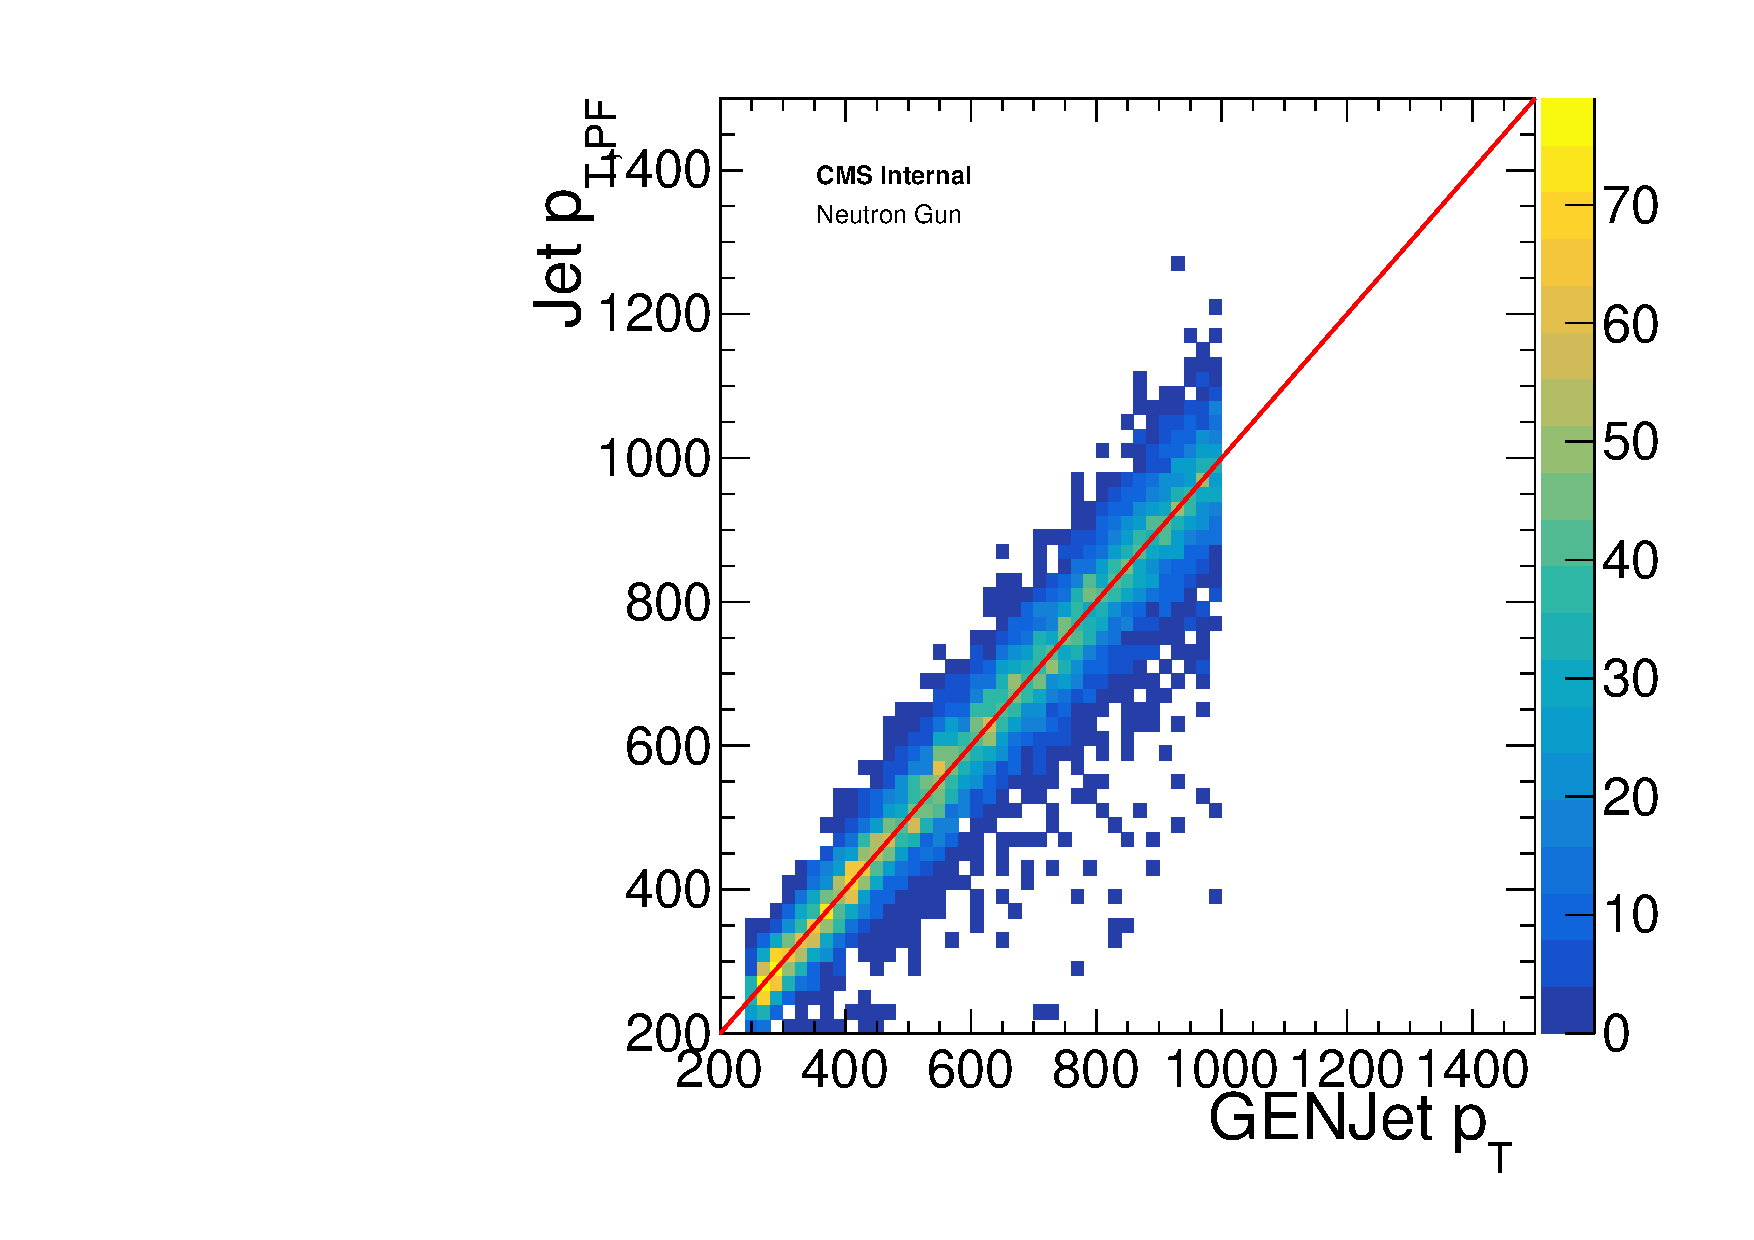
\includegraphics[width=.48\textwidth]{pt_neutron_gun_th2f_JECs_GetRandom2.pdf} \hfill
% 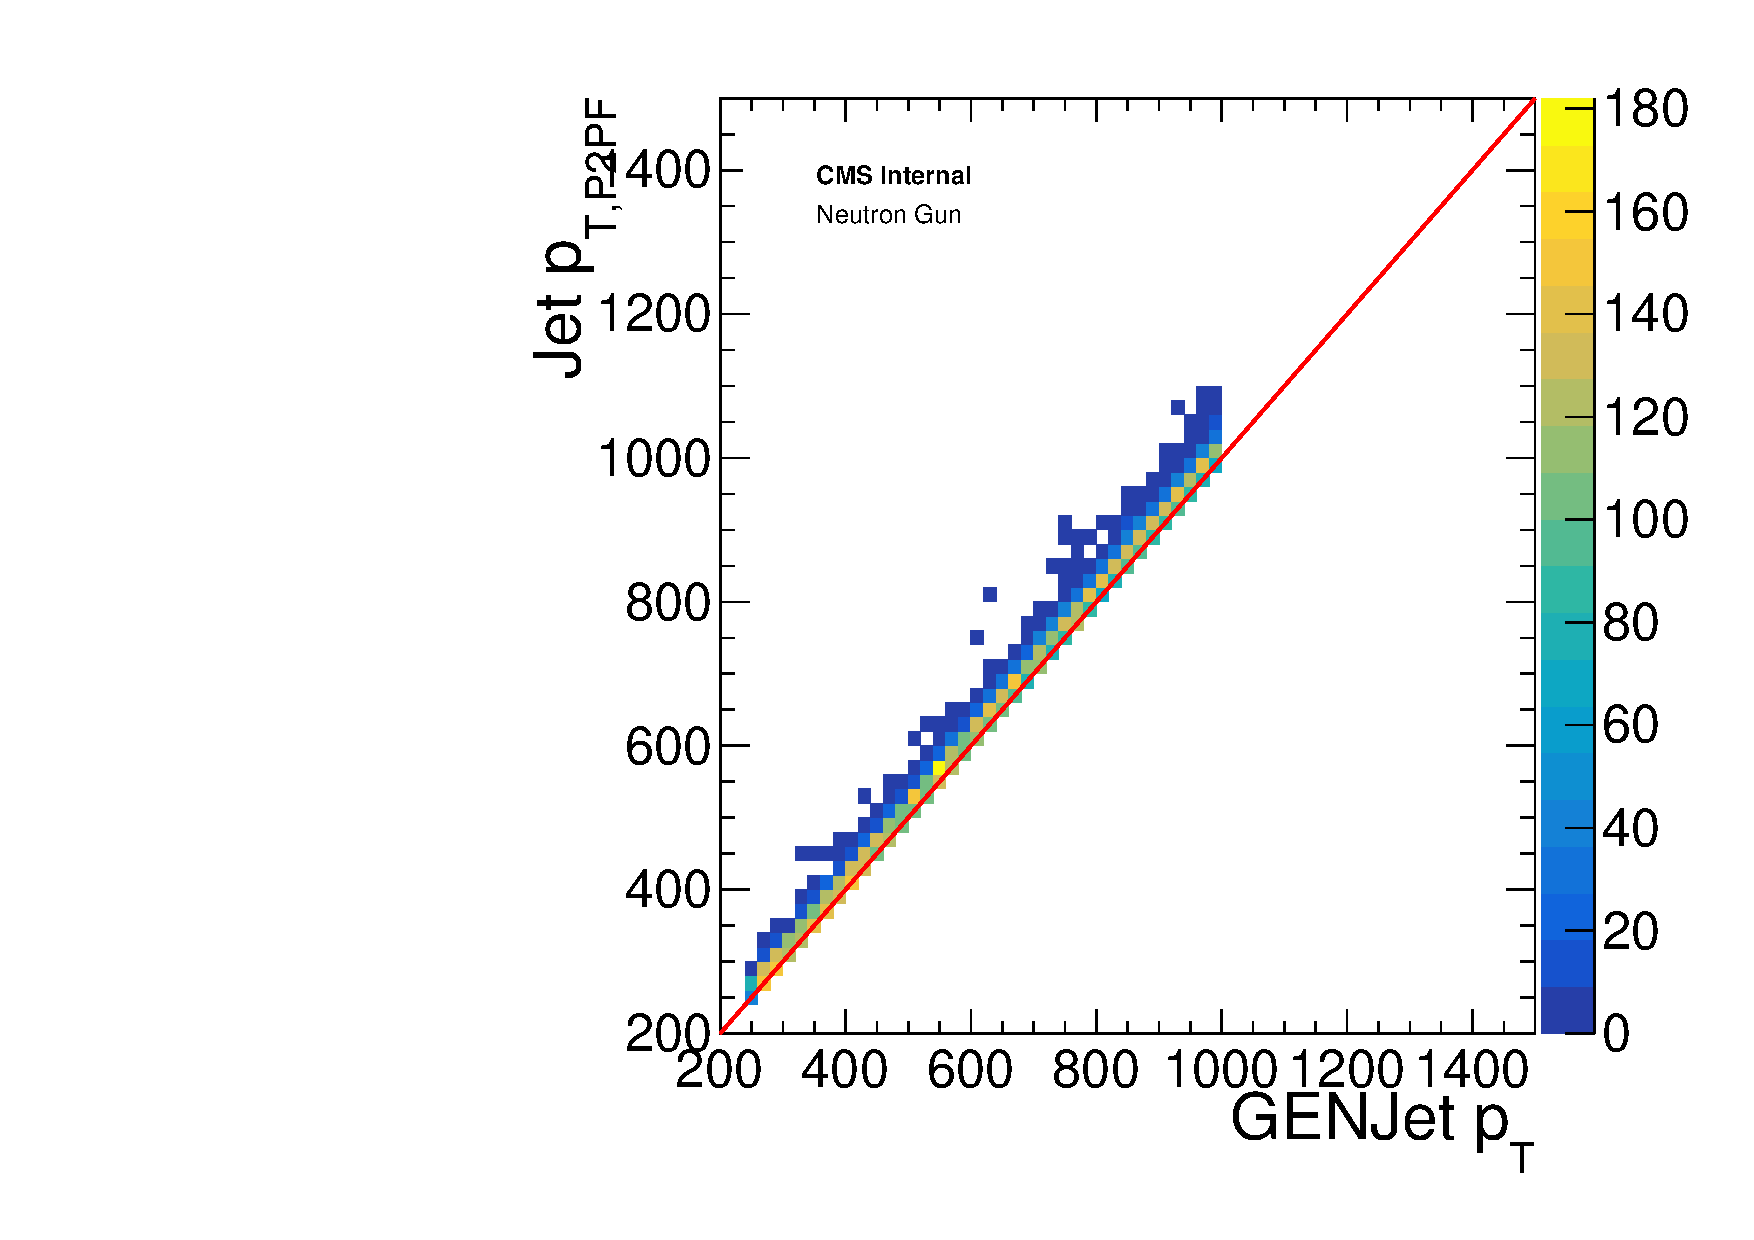
\includegraphics[width=.48\textwidth]{pt_neutron_gun_p2pf_th2f_NoSmearing.pdf}
%  \caption{Comparison of the transverse momentum of the generator-level jets to the \ac{PF} jets (left) and P2PF jets (right) without jet energy resolution smearing, using a neutron sample.}
%  \label{fig:neutron}
% \end{figure}

\begin{figure}[ht]
  \centering
 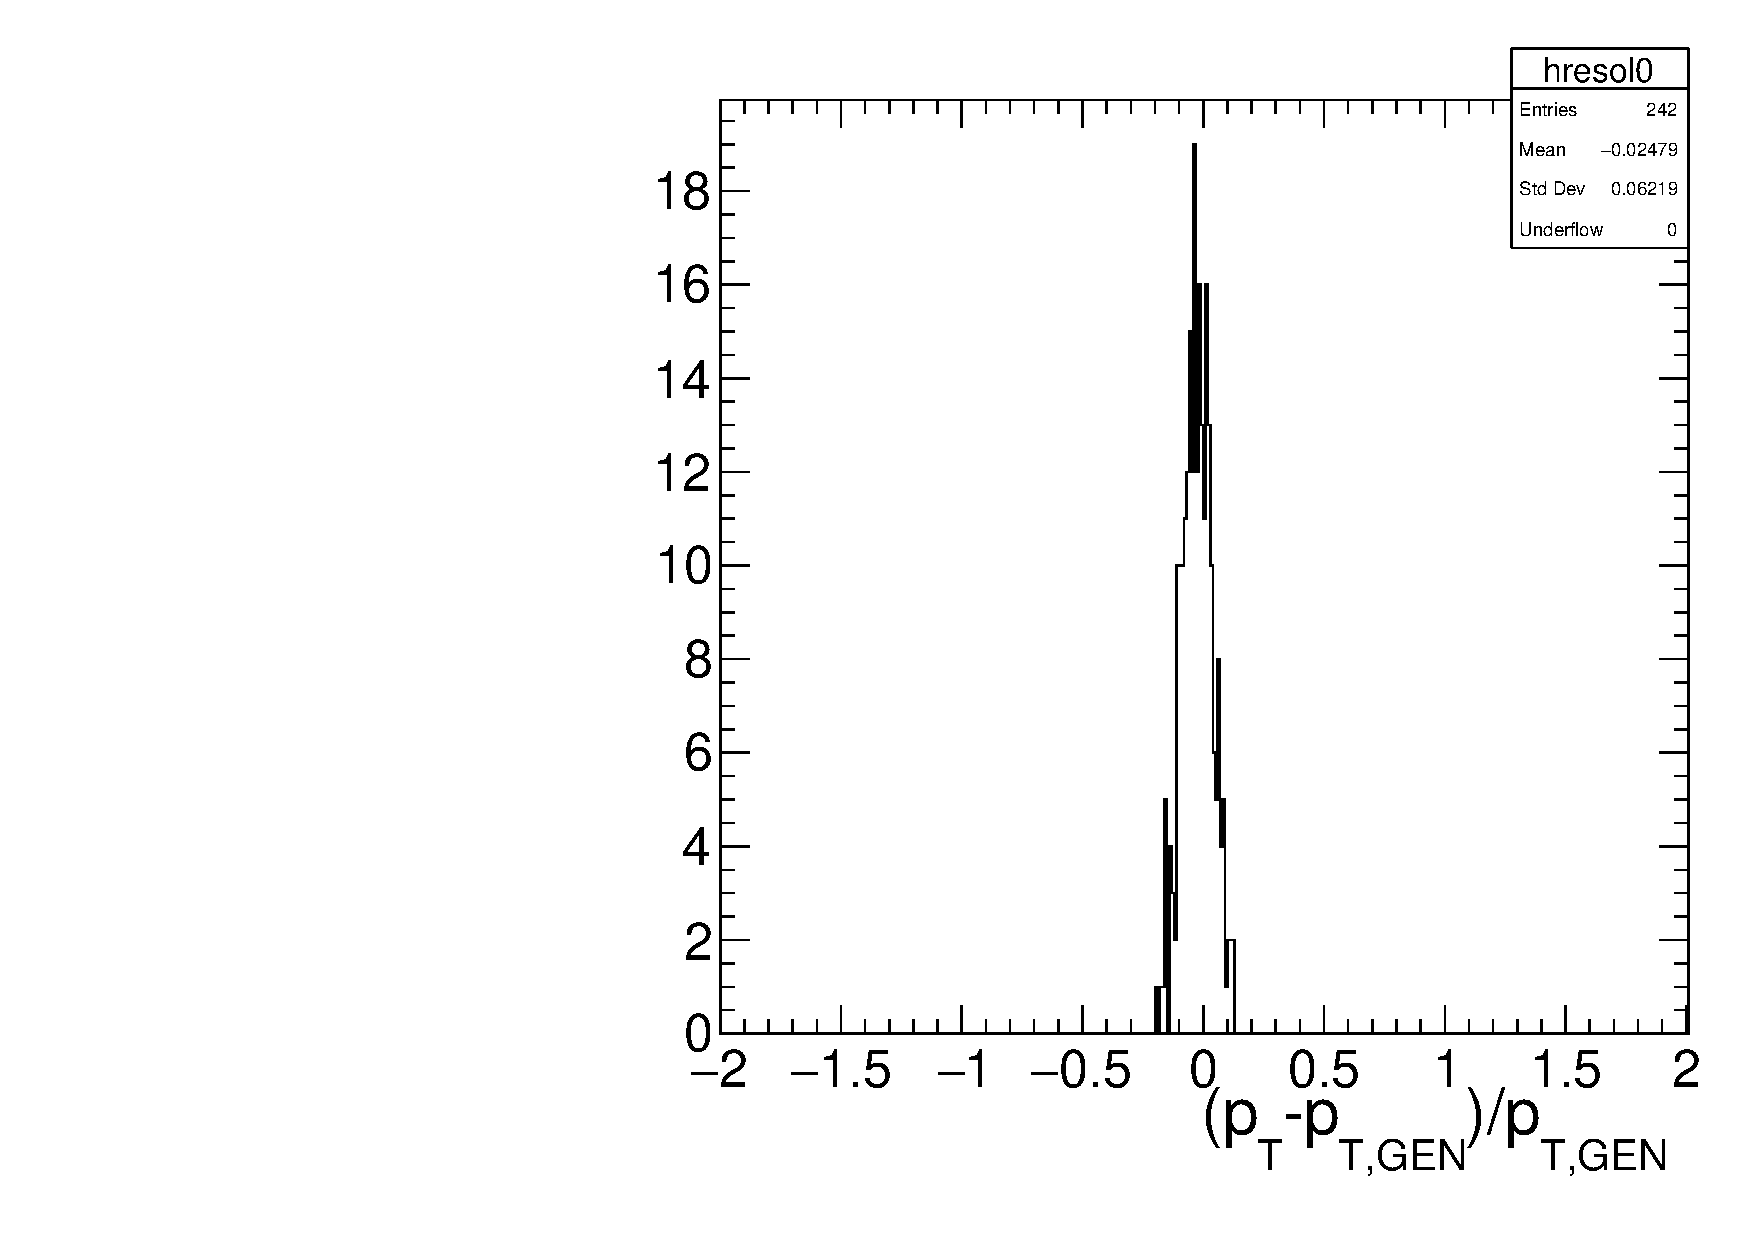
\includegraphics[width=.48\textwidth]{pt_res_ptbin_0.pdf} \hfill
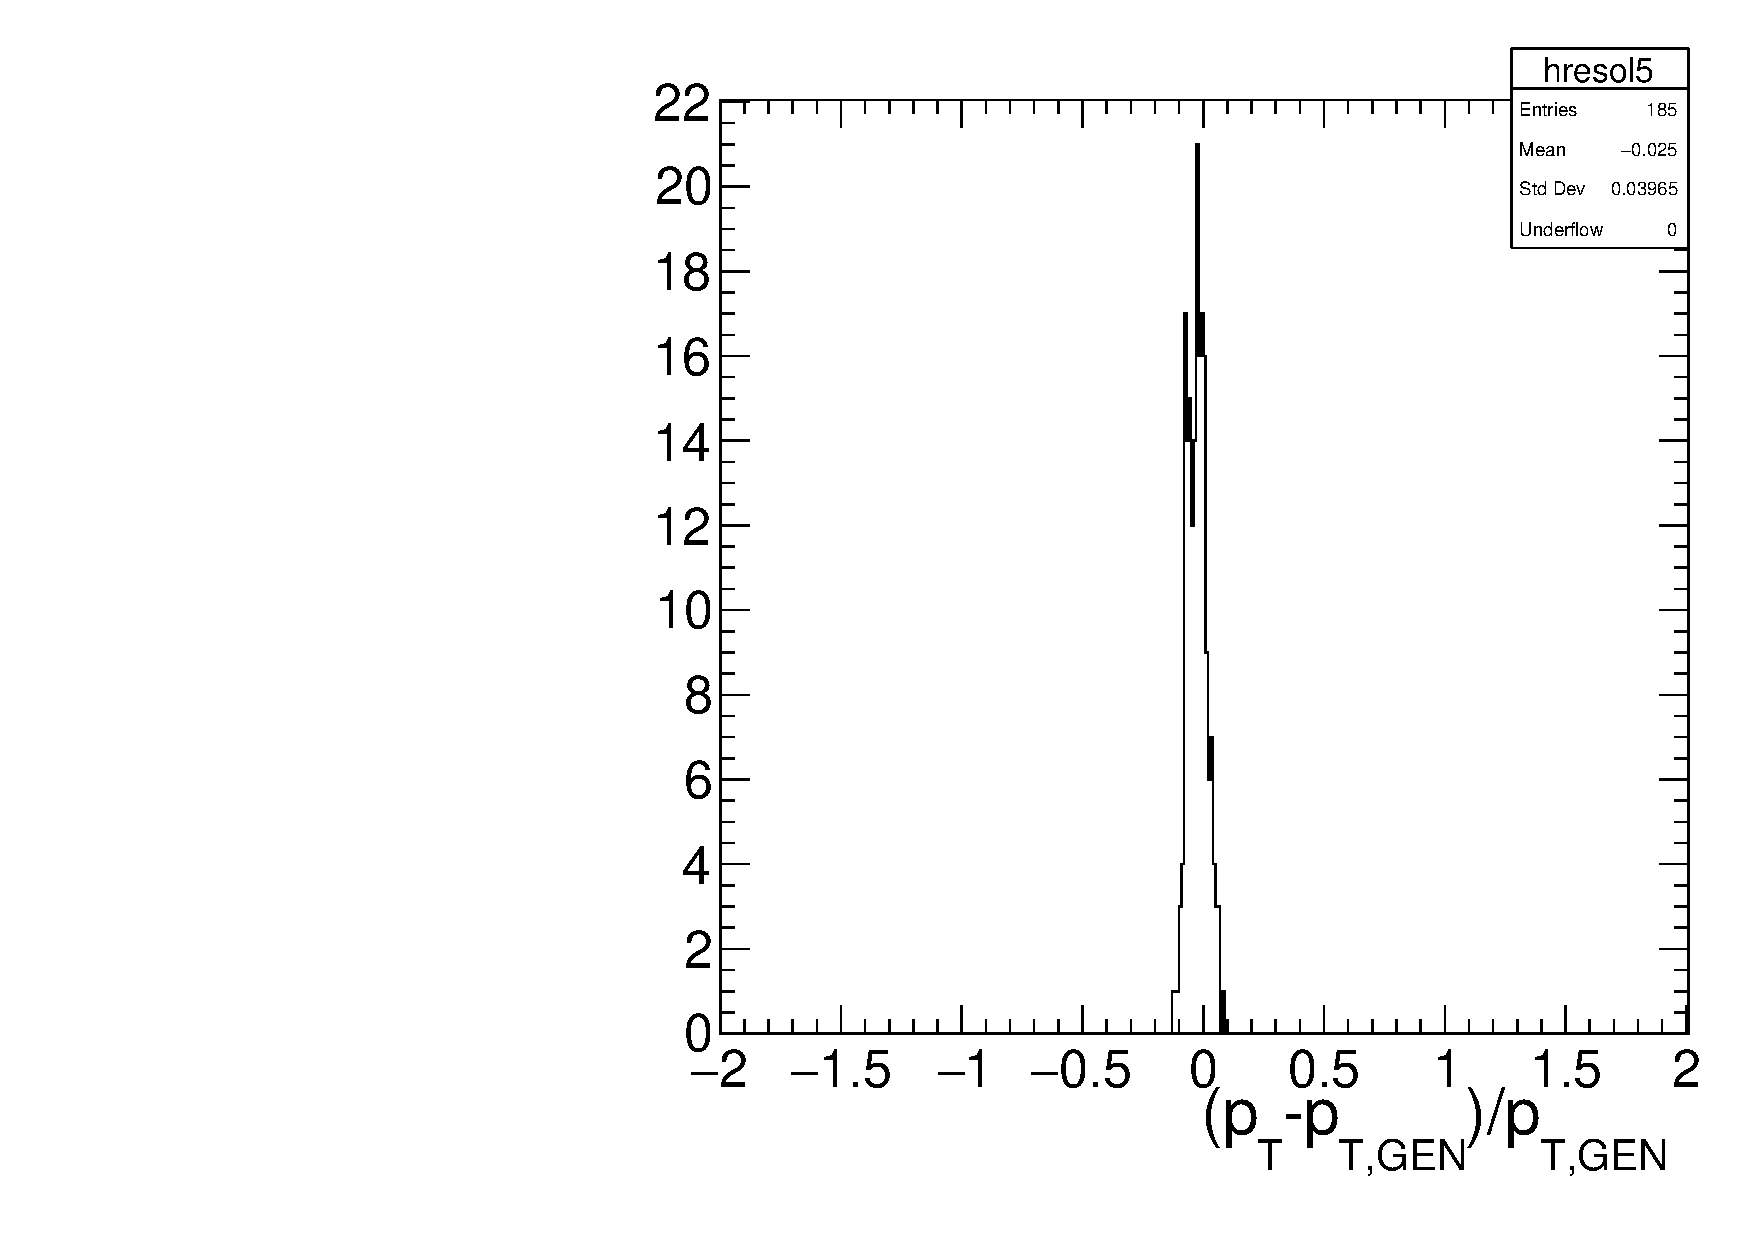
\includegraphics[width=.48\textwidth]{pt_res_ptbin_5.pdf}
 \caption{The jet energy resolution of neutrons with $0< |\eta| < 0.5$ and \SI{200}{GeV}$<p_T<$\SI{300}{GeV} (left) or \SI{700}{GeV}$<p_T<$\SI{800}{GeV} (right).}
 \label{fig:neutron_res}
\end{figure}

In order to validate this method, the custom and standard neutron samples are used to compare the two leading generator-level jets to the new jets from the custom sample, denoted as P2PF jets, and the \ac{PF} jets from the standard sample. This is illustrated in Figure~\ref{fig:neutron_corr}, where the $p_T$ of the generated neutrons is shown on the horizontal axis, and the $p_T$ of the reconstructed jet is shown on the vertical axis. The left plot shows the standard neutron sample produced with the full \textsc{Geant} simulation, while the right plot shows the custom neutron sample where the neutron was directly converted into a neutral \ac{PF} candidate. The \ac{JER} distributions are also compared in Figure~\ref{fig:neutron_res_corr} and fitted with a Crystal Ball function, showing compatible parameters.

\begin{figure}[ht]
  \centering
 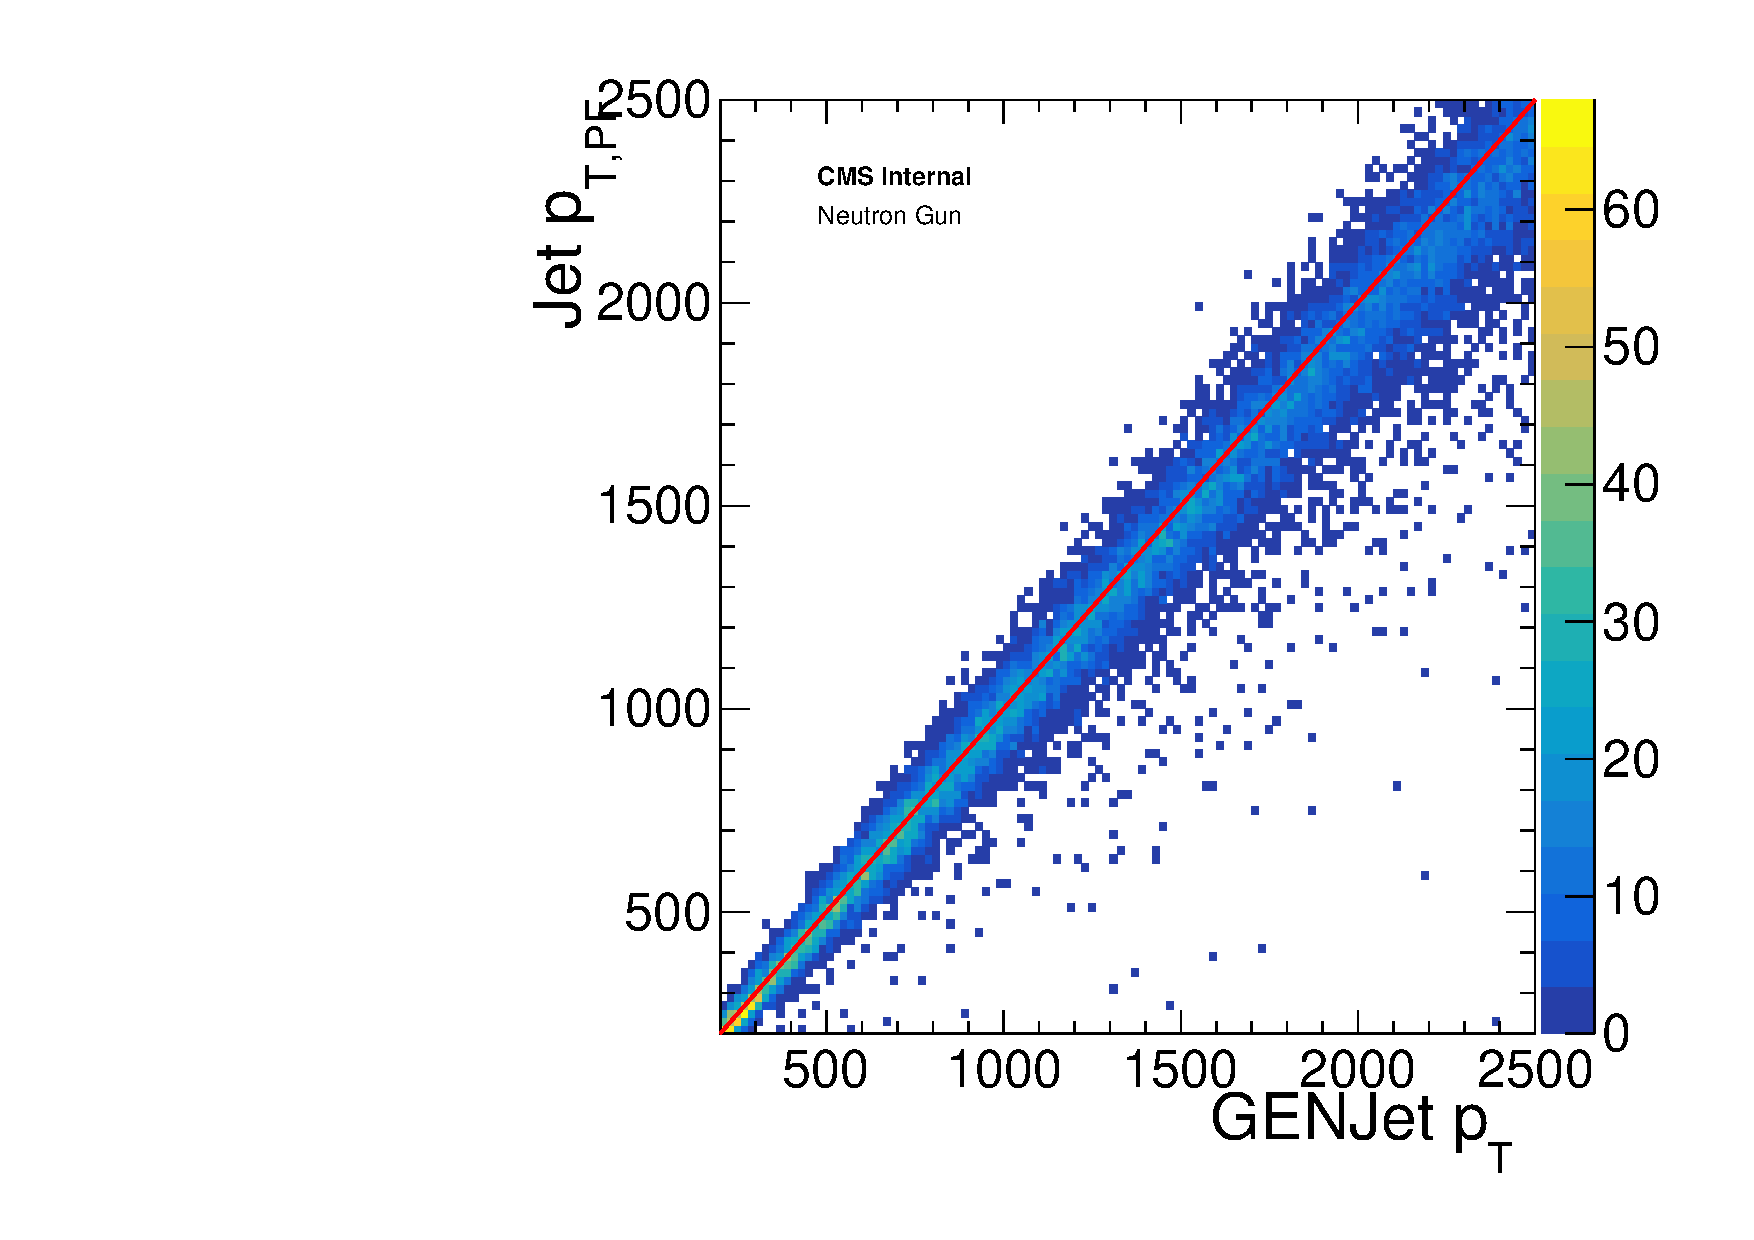
\includegraphics[width=.48\textwidth]{pt_neutron_gun_th2f_005.pdf} \hfill
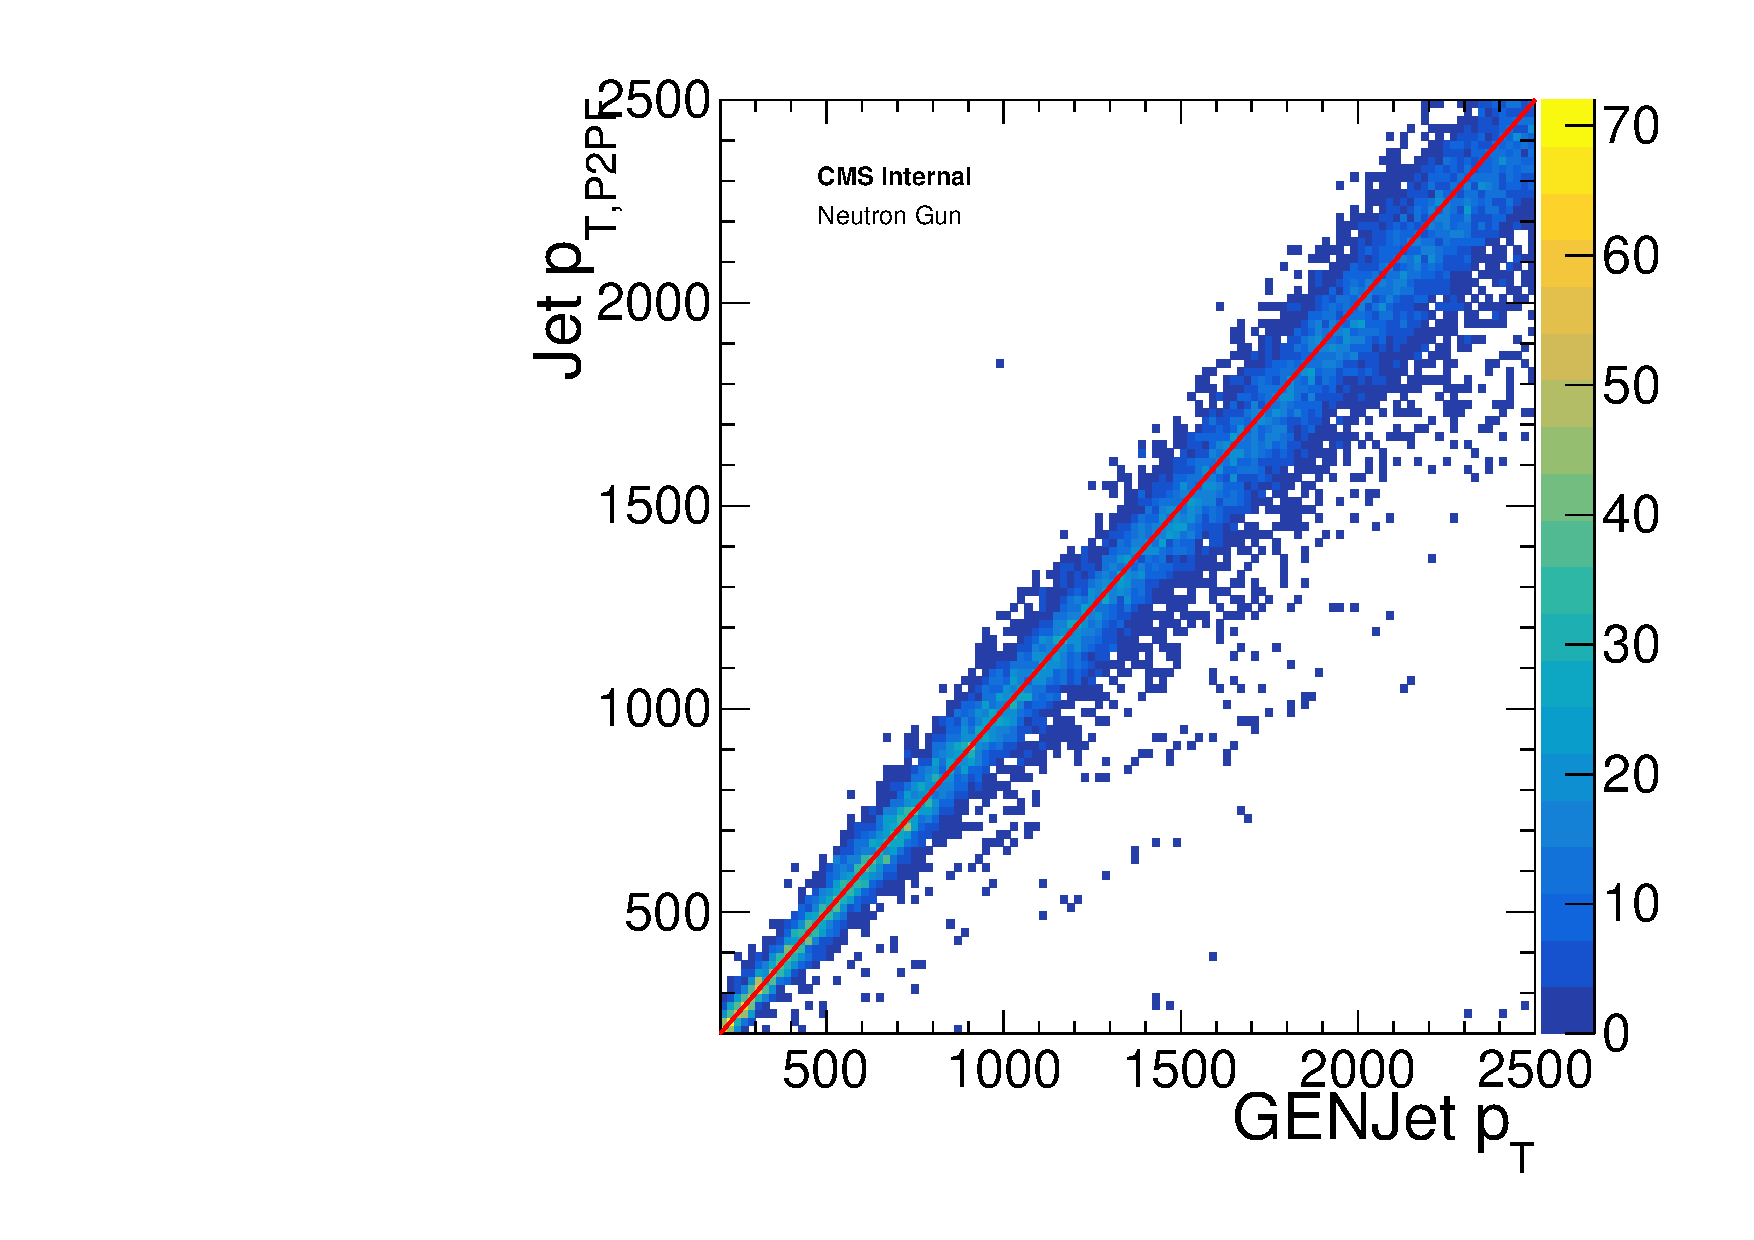
\includegraphics[width=.48\textwidth]{pt_neutron_gun_p2pf_th2f_005.pdf}
 \caption{Comparison of the transverse momentum of the generator-level jets to the \ac{PF} jets (left) and P2PF jets (right) in the region $0< |\eta| < 0.5$ with jet energy resolution smearing, using a neutron sample.}
 \label{fig:neutron_corr}
\end{figure}

\begin{figure}[ht]
  \centering
 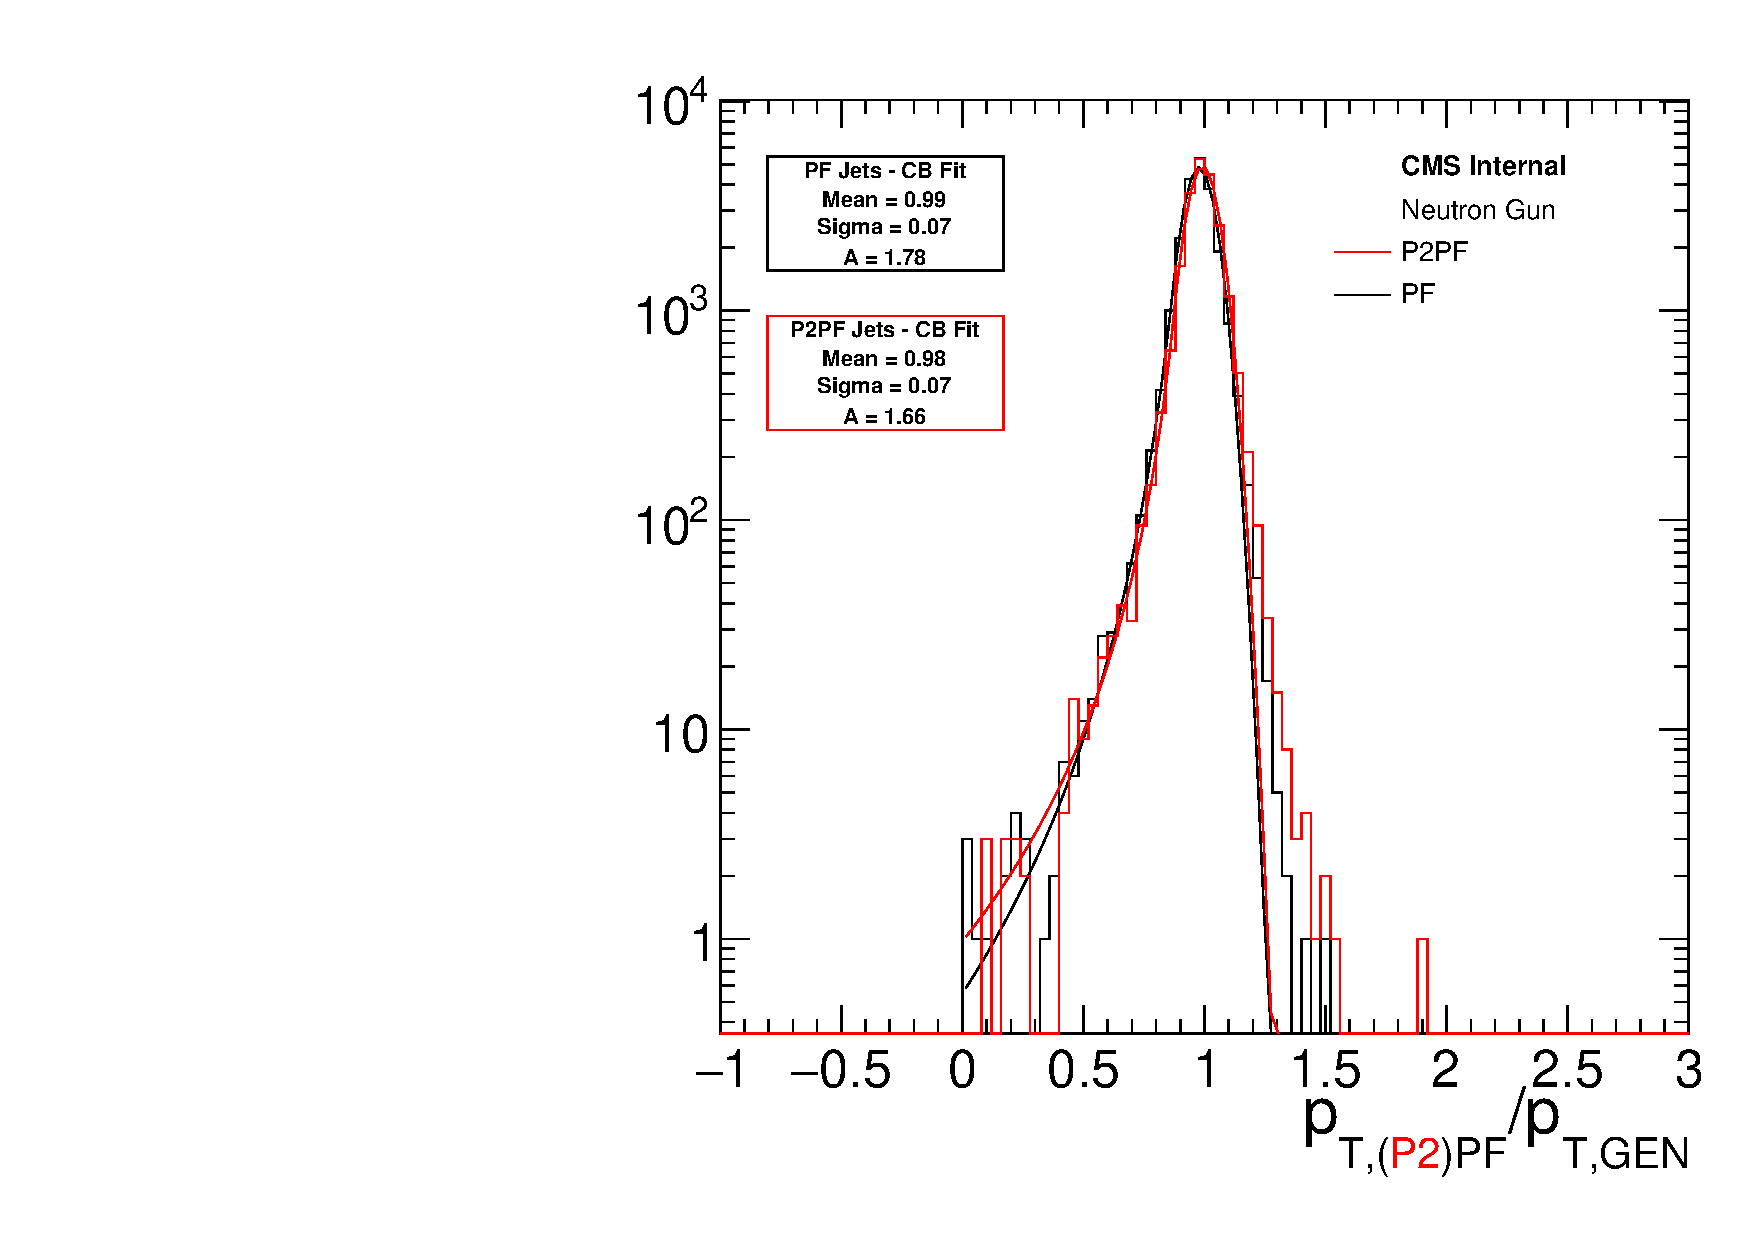
\includegraphics[width=.75\textwidth]{pt_neutron_gun_res_fit_005.pdf} 
 \caption{The jet energy resolution of the corrected P2PF jets (red) and \ac{PF} jets (black), fitted with a Crystal Ball function.}
 \label{fig:neutron_res_corr}
\end{figure}

This demonstrates that the procedure, where the \ac{JER} distributions derived from a neutron sample are used to smear the \ac{PF} candidates from generator-level \acp{SIMP}, can sufficiently accurately simulate \acp{SIMP} in a realistic detector, assuming \acp{SIMP} are neutron-like. However, since this procedure directly converts the generated \acp{SIMP} into \ac{PF} candidates, the \acp{SIMP} do not interact in the Tracker and the resulting jets have a very steeply falling charged hadron energy fraction (CHF) distribution. This gives an optimistic image, which translates in a maximal signal efficiency.

The \ac{SIMP} signal simulation and reconstruction was therefore further improved by moving to the second approach. In this method, the generated \ac{SIMP} particles are not converted into neutral \ac{PF} candidates, but they are instead replaced by neutrons, keeping the \ac{SIMP} kinematics. The standard reconstruction and full \textsc{Geant} simulation can then be applied, since the neutrons are correctly recognized and simulated. In this case, interactions will happen inside the Tracker as well and the resulting jets will contain a larger CHF, as is shown in Figure~\ref{fig:neutron_chf}. Eventually, this second method will be used in the trackless jets analysis described in Chapter~\ref{ch:SIMPs}.
 
\begin{figure}[ht]
  \centering
 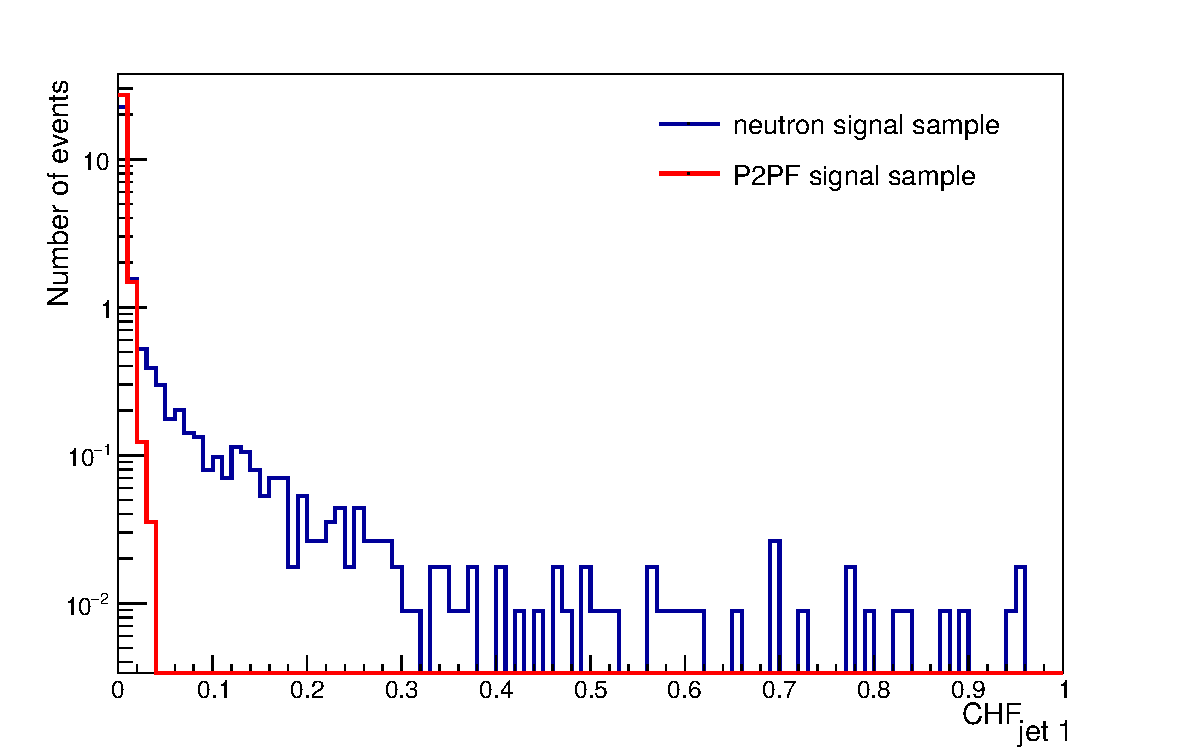
\includegraphics[width=.75\textwidth]{ChF_neutrons.pdf} 
 \caption{CHF distribution of the leading jet, for a signal sample produced with the first approach (red) and the corresponding sample produced using the second method (blue).}
 \label{fig:neutron_chf}
\end{figure}

This method gives a good approximation of a \ac{SIMP} signal, since the shower generated by the \ac{SIMP} is in principle contained inside the calorimeters, as the model described in Section~\ref{sec:SIMP} is constructed so that for a specific choice of couplings the \acp{SIMP} may be detected as regular hadrons. Although the considered \ac{SIMP}-nucleon interaction is repulsive, this does not differ considerably from known attractive interactions at the probed high energies. The incoming \ac{SIMP} hits a nucleon at rest in the calorimeter, breaking it up, and because of the large incoming momentum, there is a boost forward into the calorimeter and the shower starts. The cross section would therefore be identical for a repulsive or attractive interaction and the effect on the shower is negligible since the scattering angle is very small due to the momentum boost. Furthermore, the higher the momentum of the \ac{SIMP}, the shorter the distance it travels to deposit its characteristic momentum. With the considered couplings, the depth containing a \ac{SIMP} with \SI{500}{GeV} momentum is below \SI{1}{m}, within the calorimeter~\cite{Bryan}. Most of the energy will therefore be deposited in the first interaction with the material. Given the expected forward energy flow in the calorimeter shower, and the shower containment achieved by the choice of couplings in the simplified model, the shower induced by the \ac{SIMP} interaction can to first order be modelled by the interaction of a high-momentum neutral hadron, like a neutron.

\clearpage
\clearpage{\pagestyle{empty}\cleardoublepage}
